\documentclass[11pt]{article}
\usepackage{geometry}
\geometry{
    a4paper,
    total={6in,9in}
    }

\usepackage{mathtext}
\usepackage{float}
\usepackage{booktabs}
\usepackage{amsmath}
\usepackage{amssymb}
\usepackage{mathtools}
\usepackage{calligra}
\usepackage{color}
\usepackage{authblk}
\usepackage{textcomp}
\usepackage{graphicx}
\usepackage{booktabs}
\usepackage{xcolor}
\usepackage{array}
\usepackage{colortbl}
\usepackage{textcomp}
\usepackage{tabularx}
\usepackage{tabulary}
\usepackage[colorlinks = true,
            linkcolor = blue,
            urlcolor  = blue,
            citecolor = blue,
            anchorcolor = blue]{hyperref}


%Colors
\definecolor{darkspringgreen}{rgb}{0.09, 0.45, 0.27}
\definecolor{lightblue}{RGB}{212,236,244}

%formats that look like standard dune tables
\newcommand{\rowtitlestyle}{
  \rowcolor{lightblue}
  %\rowstyle{\bfseries \boldmath} 
}

\newcommand{\colhline}{
  \arrayrulecolor{gray}
  \specialrule{0.5pt}{0pt}{1pt}
  \arrayrulecolor{black}
}

\newcommand{\toprowrule}{
  \arrayrulecolor{gray}
  \specialrule{1.2pt}{0pt}{1pt}
  \arrayrulecolor{black}
}


\newcommand*\app{\raise.17ex\hbox{$\scriptstyle\mathtt{\sim}$}}
\newcommand{\overbar}[1]{\mkern 1.5mu\overline{\mkern-1.5mu#1\mkern-1.5mu}\mkern 1.5mu}
%%\graphicspath{ {\string~/Box Sync/Presentations/PTB_MTCA_SBND/VerticalSlice/figures/} }
\graphicspath{{./fig/}}

%opening
\title{\vspace*{\fill} \textbf{Data Selection for DUNE Beam and Atmospheric Events}}
\author[1]{David Last} 
\author[1]{David Rivera} 
\affil{University of Pennsylvania}


\begin{document}
\maketitle
\mbox{}
\vspace*{4in}
\newpage


\maketitle

\section{Motivation}
For DUNE's main physics program to be achievable, it is required that the trigger be practically 100\% efficient at, and above, 100 MeV visible energy, as to meet the requirement set in %DUNE CDR. 
. Furthermore, the rate of fake triggers should not exceed the rate of cosmic events in the detector, as to limit the data processing rates to acceptable levels. The current structure of the DUNE triggering system is such that primitives are processed at an APA-level to generate trigger candidates. These candidates are then processed by a module-level trigger and if the decision is made to trigger, the data for the entire module is written out for a 2-drift sized window centered around the time the trigger was issued (see~\href{https://docs.dunescience.org/cgi-bin/private/ShowDocument?docid=9240}{DUNE-doc-9240}).
The focus of this document is on the candidate generation algorithms. Supernova events are triggered via a different schema which relies on a large data buffer. From this fact, the focus of this document is consequently on DUNE's ability to trigger on Beam and Atmospheric events. The algorithms are generic with the goal that they apply to other sources of data of interest for DUNE e.g. solar neutrinos and cosmics.

The guiding assumption that pervades the studies discussed here is that for every trigger candidate generated, a module-level trigger will be issued. This means (based on an estimated cosmic event rate of 1000/day
) that the maximum acceptable rate of fake triggers from radiological backgrounds (as this will dominate the overall trigger rate) is as follows:
\begin{align*}
    \frac{1000}{\text{day}*\text{module}}\cdot\frac{1\text{module}}{150\text{APA}}\cdot\frac{1\text{day}}{24 \text{hr}*3600\text{sec}/\text{hr}}\approx 77\mu \text{Hz}/\text{APA}
\end{align*}
The studies outlined in this document look to limit the rate to $7.7\mu$Hz/APA as to potentially be stable against variations in radiological and random-noise rates. Argon-39 is expected to be the primary radiological contribution by rate. It was determined that Argon-39 pileup was well-mitigated by breaking up a drift into 50$\mu$sec windows (see~\href{https://docs.dunescience.org/cgi-bin/private/ShowDocument?docid=9808}{DUNE-doc-9808}) using a Toy Model. Therefore, this was taken to be the candidate generation window.


\section{Algorithms}

Significant efforts have been made in the department of generating trigger primitives from raw waveforms for the collection plane (see~\href{https://wiki.dunescience.org/wiki/Tools_for_2018_Trigger_Primitive_Studies}{Phil Rodrigues's wiki}), and our work has focused on taking those primitives and issuing APA-level trigger candidates from them.
Implementation of the aforementioned trigger primitives into our studies has yet to be performed.

The complete stream of processing the data to generate candidates is as follows:

\begin{center}
Hit Finding $\rightarrow$ Clustering $\rightarrow$ Trigger Candidate Finding    
\end{center}

Simulated data samples, including Monte Carlo Challenge (MCC) datasets, are first reconstructed utilizing the RawHit Finder class which returns a channel-ordered series of hits for the entire drift. The RawHits are produced anytime the raw waveforms cross the desired threshold. For collection signals, the RawhHit objects contain the following variables of interest: 
\begin{itemize}
\setlength\itemsep{0em}
    \item \textbf{time}: Start Tick, End Tick, Peak\_Time, Sigma\_Peak\_Time, 
    \item \textbf{amplitude}: Peak\_Amplitude, Summed Charge 
\end{itemize}

where the Start and End Ticks correspond to the time at which the waveform crossed a pre-defined threshold in the positive and negative direction, respectively. Prior to processing hits, these are sorted into time bins corresponding to candidate generation windows. 
\textbf{Note:} Collection signals, alone, cannot distinguish between ionization events observed along the vertical direction; this would require induction wires. 


The total charge (Summmed ADC) captured in a single TPC per APA (whichever had more is used), is considered as the primary parameter on which to issue a trigger candidate. The decision for issuing a candidate is further parametrized into a basis composed of the spread in z (Adjacency/Cluster Size), time (Time-Over-Threshold), and total charge (Wire Summed ADC). This basis was chosen %as a starting point
given the following arguments: 

\begin{enumerate}
\setlength\itemsep{0em}
    \item tracks in the $\pm$\textbf{z} (beam) direction will produce hits across multiple adjacent wires
    \item tracks in the $\pm$\textbf{x} (drift) direction tend to produce signals which extend in the time direction and hence could be identified by the time over threshold
    \item the charge from tracks in the $\pm$\textbf{y} direction and parallel to the wires will be collected by one or two wires over a small time window resulting in larger amplitude signals
\end{enumerate}

Adjacency and Cluster Size are defined in the following paragraphs. The Time-Over-Threshold is simply the time difference between the End and Start ticks of a hit, and the maximum per candidate generation window is utilized to make the decision. The maximum summed ADC of a single hit is similarly the defined Wire Summed ADC parameter used in the decision.

The first method utilized to cluster hits is referred to as Adjacency, and it requires counting the number of adjacent collection wires for which a hit was found in the candidate window. As with the other variables above, the maximum in the window is taken to be the parameter on which the candidate decision is made.

Clustering is the other method utilized to group hits. This method divides the candidate generation window into ten smaller ``primitive windows", 10$\mu$s each. The adjacency in a single primitive window is calculated as above. Then, each grouping (cluster) with the highest charge in a primitive window is compared to the same such grouping in each adjacent primitive window. If the bounds of the clusters are such that any wire within one cluster is adjacent to or the same as any wire in the other cluster, they are considered connected and their adjacencies (sizes) are added. The larger number between the maximum sum of cluster sizes and the maximum single primitive window adjacency is labeled as the cluster size for that window and used as the parameter in decision making.

The current schema for issuing a trigger candidate is to only issue a candidate if at least one of the four parameters crosses a pre-determined threshold. The threshold is determined by limiting the fake trigger rate to the order of the aforementioned 7.7$\mu \text{Hz}/\text{APA}$, the details of which are discussed in the following section.

\section{Studies}

All samples generated and studied here utilize the 1x2x6 geometry in accordance with MCC simulations. This geometry represents a subset of the central portion of the full 10kt module geometry i.e. the row of APAs is surrounded on both sides by a full 3.6 meter drift. 

\begin{figure}[H]
    \centering
    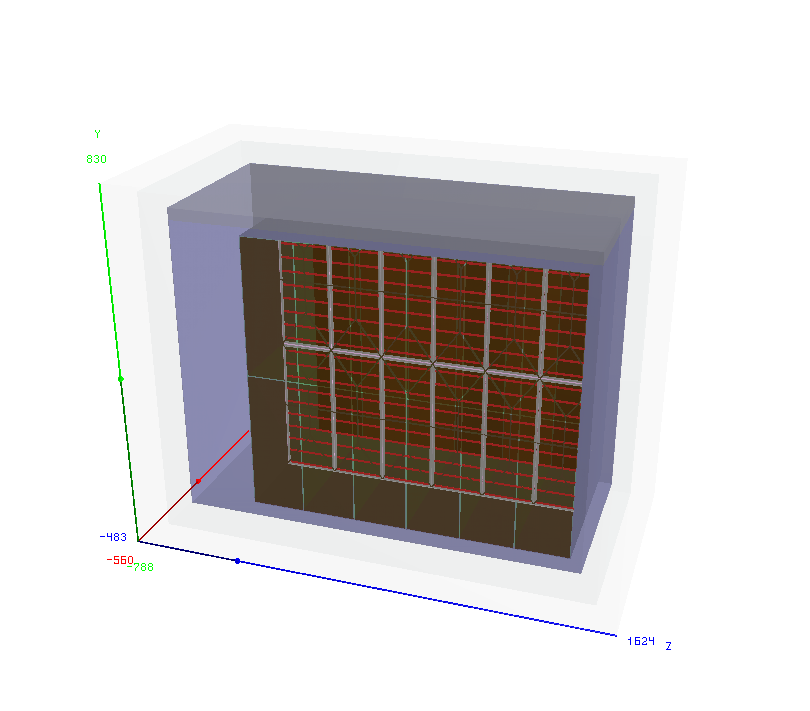
\includegraphics[width=0.7\textwidth]{dune_1x2x6_full_axes_test.png}
    \caption{1x2x6 DUNE geometry corresponding to a single row of two vertically-stacked APAs that is 6 APAs deep and centered between two CPAs.}
    \label{fig:geom}
\end{figure}

\subsection{Radiologicals}

%table that I took from my Ar39 report and reformatted
\begin{table}[h!]
\begin{center}
\caption{Simulated Backgrounds}
\begin{tabular}{ |l|l|l| }
  \toprule
  \rowtitlestyle Background & Source/Nuclide & Content (Bq/cc) \\ 
  \toprowrule 
  CPA & $^{40}$K &2.72E-3 \\ \colhline
  $^{39}$Ar & $^{39}$Ar & 1.41E-3 \\ \colhline
  $^{85}$Kr &$^{85}$Kr &  1.60E-4 \\ \colhline
  APA & $^{60}$Co & 8.20E-5 \\ \colhline
  $^{222}$Rn & $^{222}$Rn & 5.58E-5 \\ \colhline
  Neutron & Concrete & 3.04E-5 \\ \colhline
  $^{210}$Po & $^{222}$Rn & 5.00E-6 \\ \colhline
  $^{42}$Ar & $^{42}$Ar & 1.28E-07 \\ \colhline
  %\caption{table}
\end{tabular}
\label{tab:bkg}
\end{center}
\end{table}

To determine ``keep-all" thresholds which properly limit the rate near to the desired value, it is necessary to have 0 triggers in roughly 1,000,000 events in the 12 APA, 1x2x6 Geometry. The below results were obtained by simulating 1,028,000 events with the background rates outlined in Table \ref{tab:bkg}.

\begin{figure}[H]
    \centering
    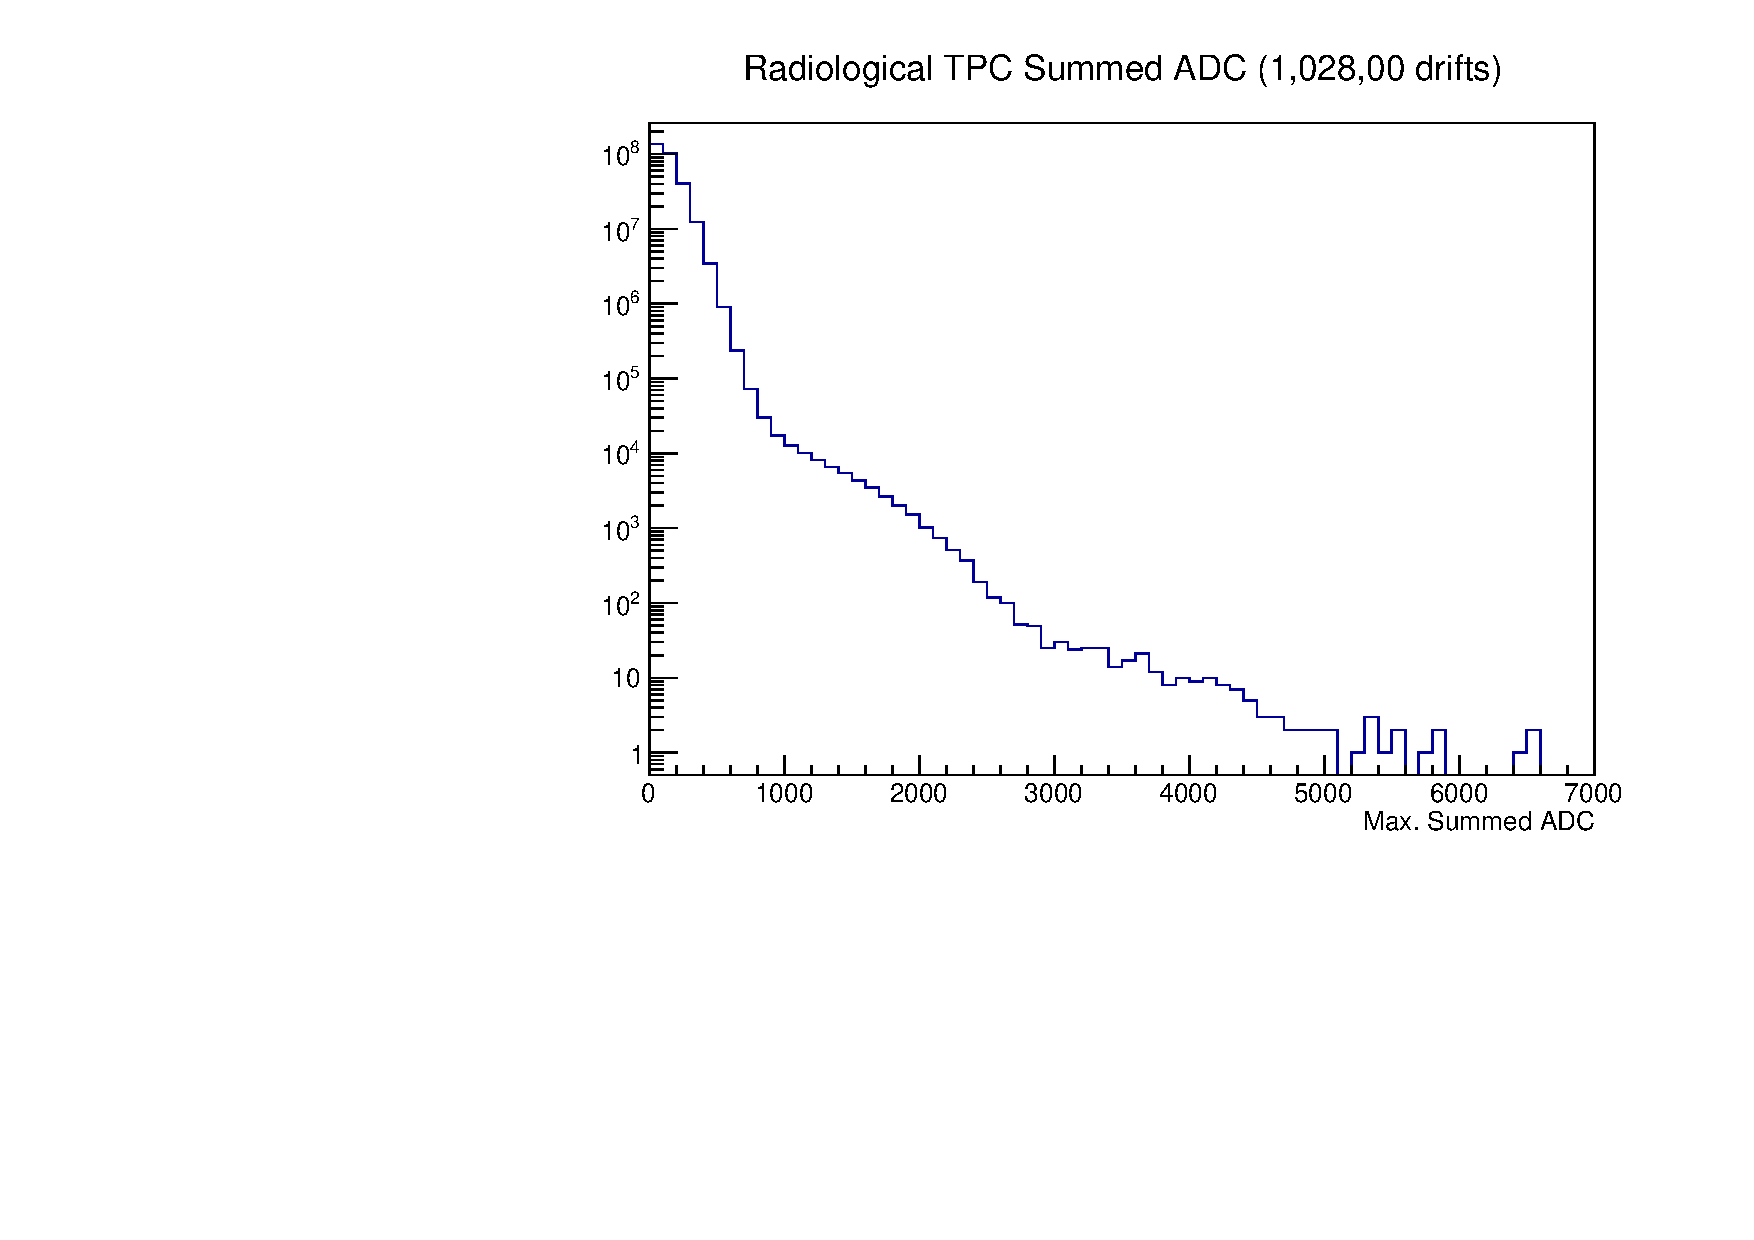
\includegraphics[angle=270,width=0.45\textwidth]{Rads/rads_TADC.pdf}
    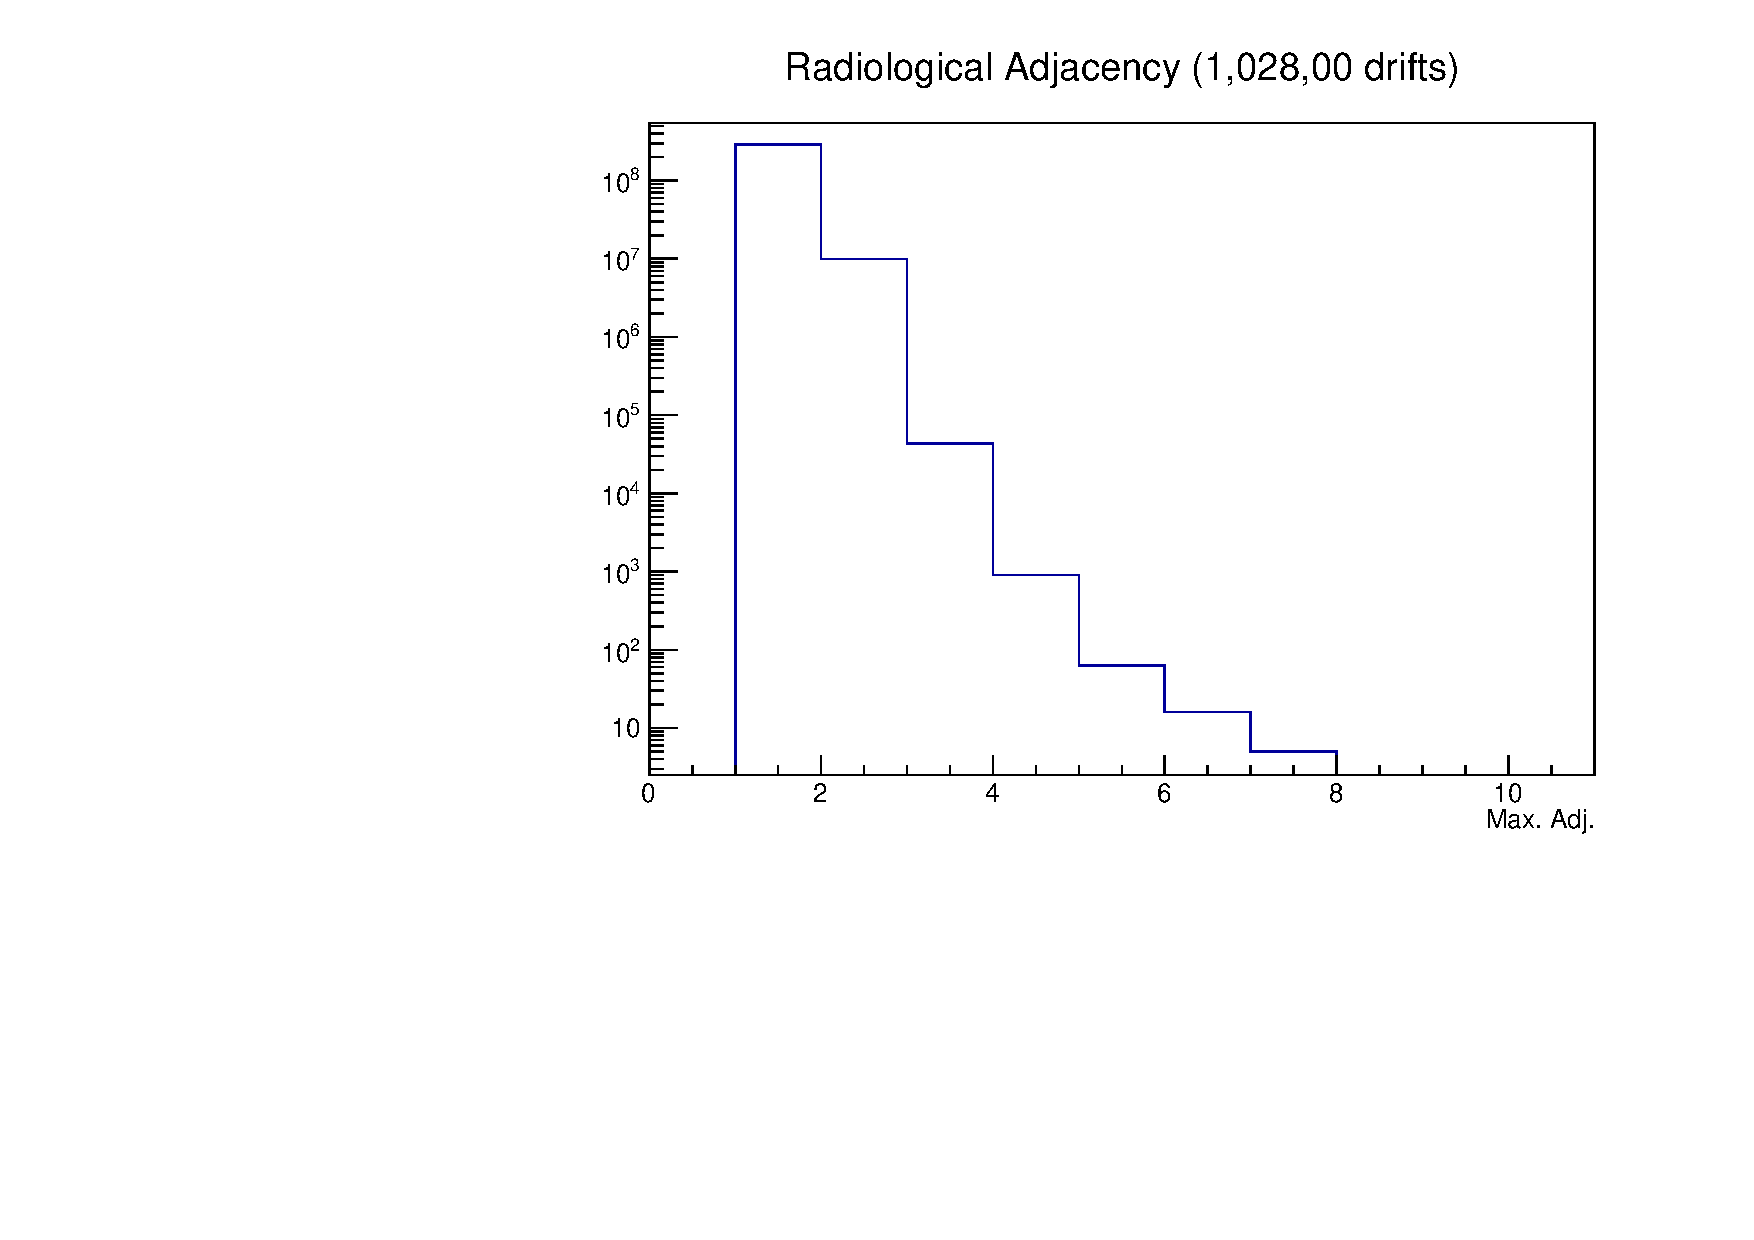
\includegraphics[angle=270,width=0.45\textwidth]{Rads/rads_max_adj_log.pdf}
    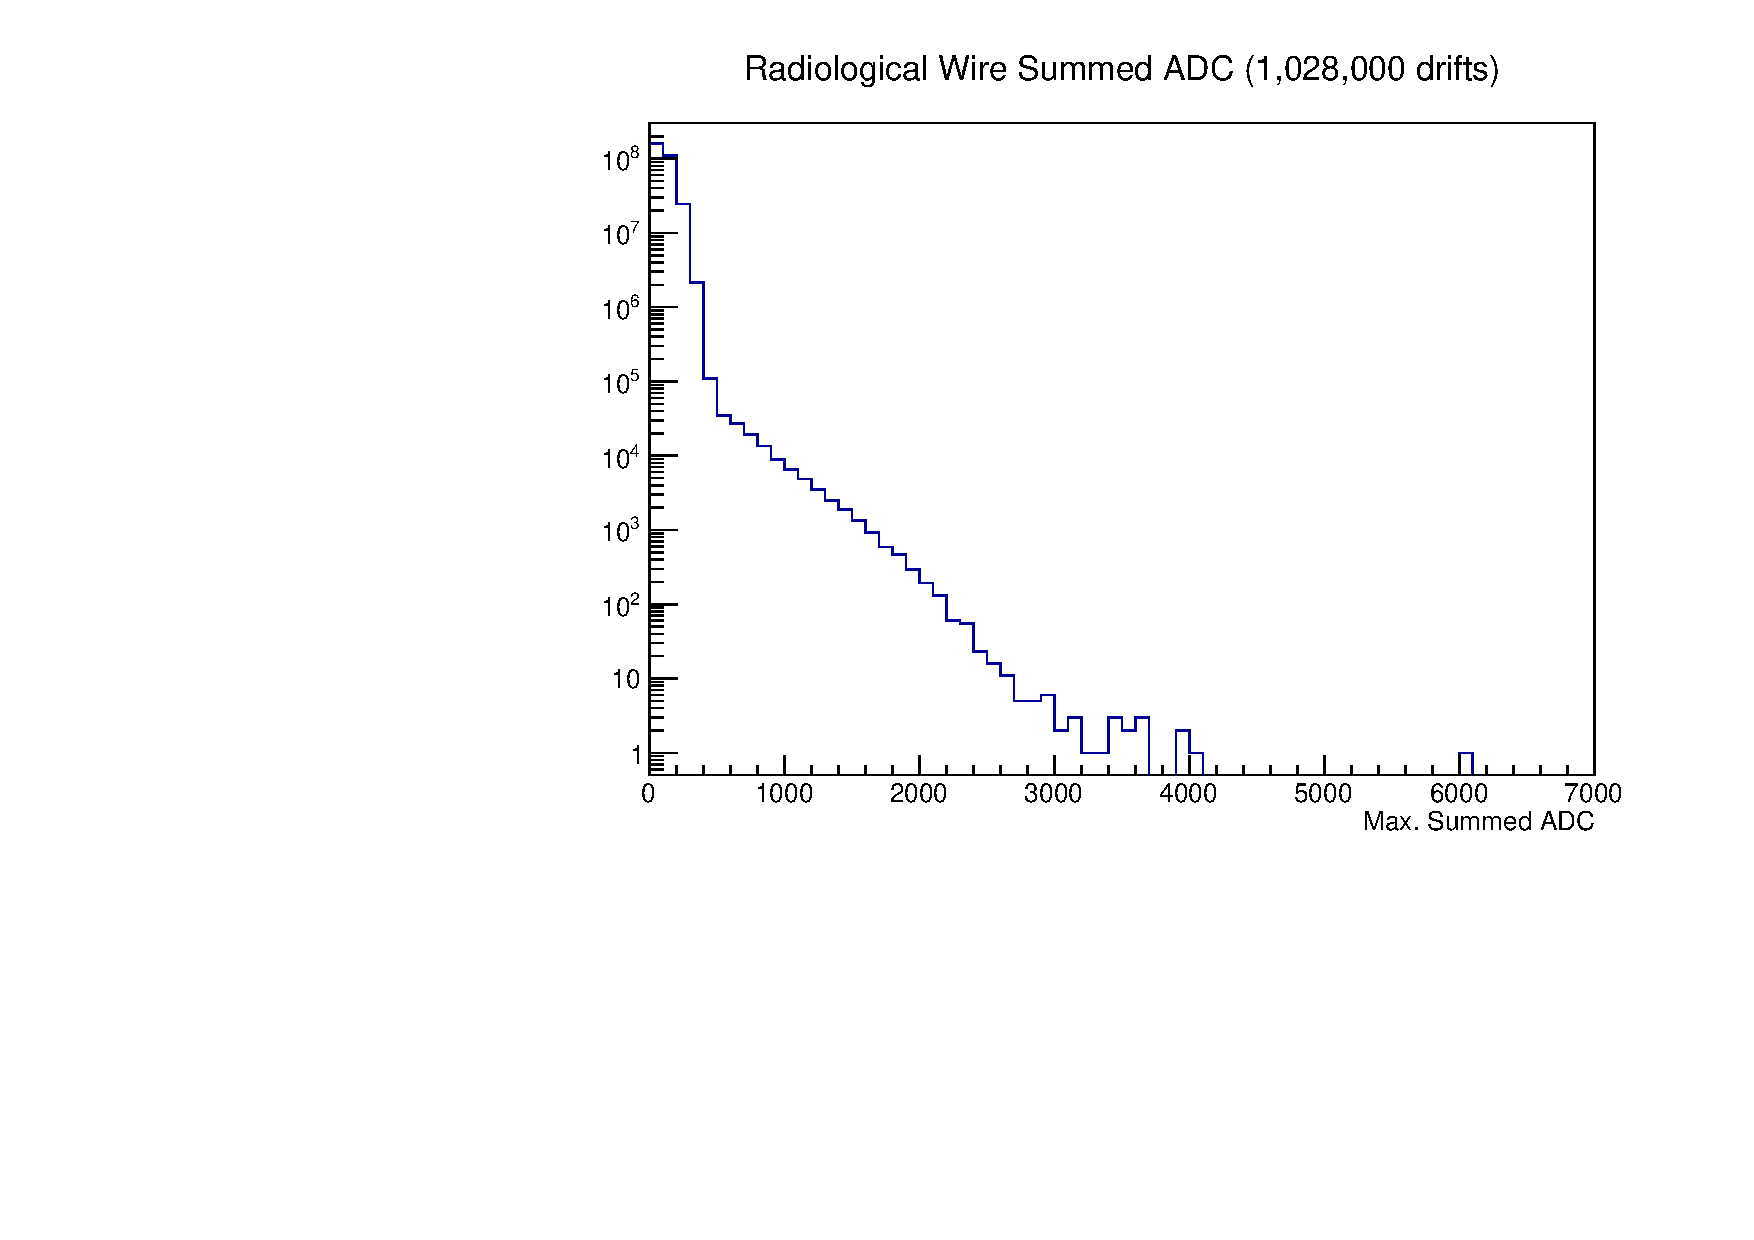
\includegraphics[angle=270,width=0.45\textwidth]{Rads/rads_WADC.pdf}
    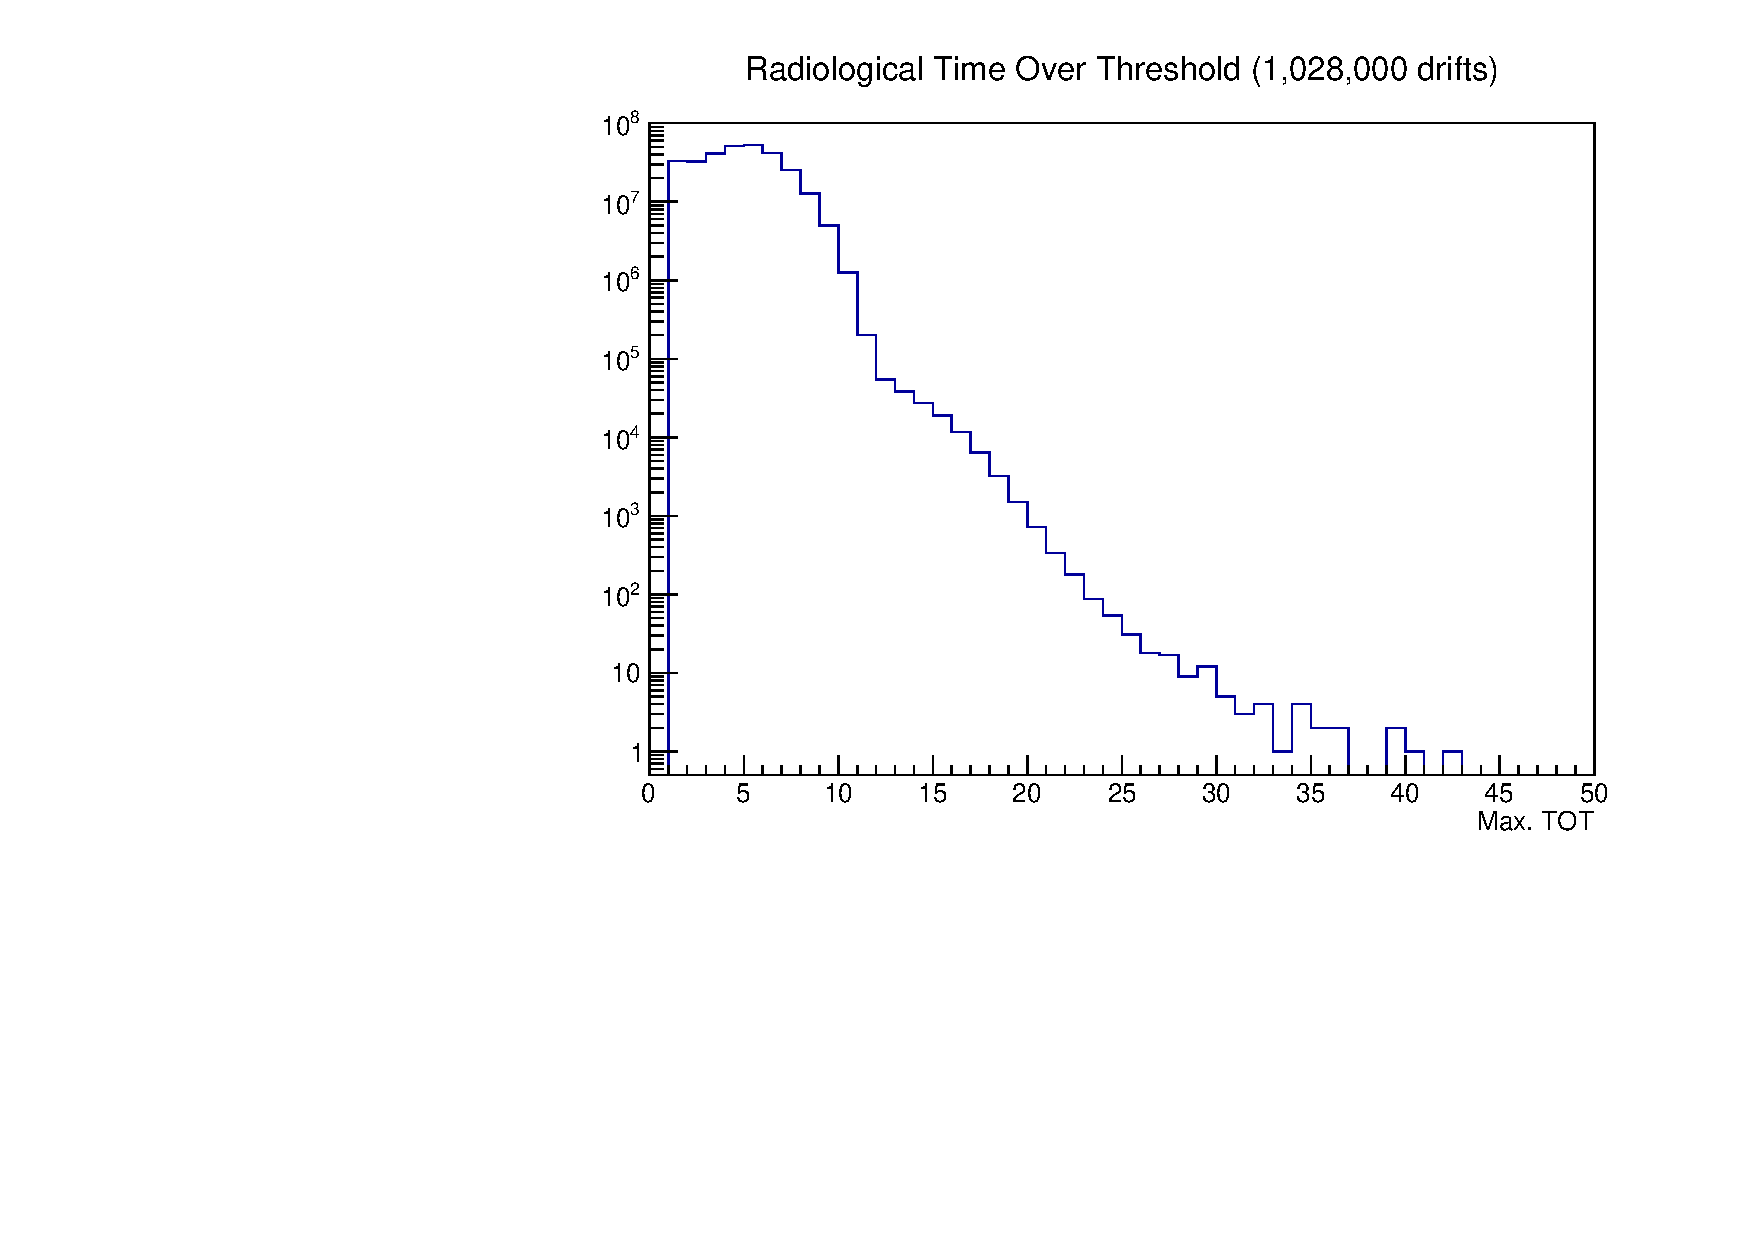
\includegraphics[angle=270,width=0.45\textwidth]{Rads/rads_TOT_log.pdf}
    \caption{Radiological distributions for trigger candidate generation variables.}
    \label{fig:eff_atm}
\end{figure}

From these plots, it was determined that the following four thresholds would sufficiently limit the rate:
\begin{itemize}
    \item Summed ADC $\geq 7000  \text{ counts}$
    \item Adjacency/Cluster Size $\geq 8$
    \item Wire Summed ADC $\geq 6500 \text{ counts}$
    \item Time Over threshold $\geq 45 \text{ ticks}$ 
\end{itemize}

\subsection{Efficiency}

The definition of efficiency was defined, \textit{a priori}, for events whose primary interaction vertex is contained within the active volume of the detector. A active volume cut on the vertex position was applied to exclude vertices extending outside of:
\begin{itemize}
    \item $\mid x \mid > 360.0$ cm
    \item $\mid y \mid > 600.0$ cm
    \item $0\text{ cm} <  z < 1390.0\text{ cm}$ 
\end{itemize}
in the 1x2x6 geometry shown in figure~\ref{fig:geom}. 

\subsubsection{Beam MCC}

The following shows the trigger efficiency as a function of Energy for the MCC10 sample of beam events.

\begin{figure}[H]
    \centering
    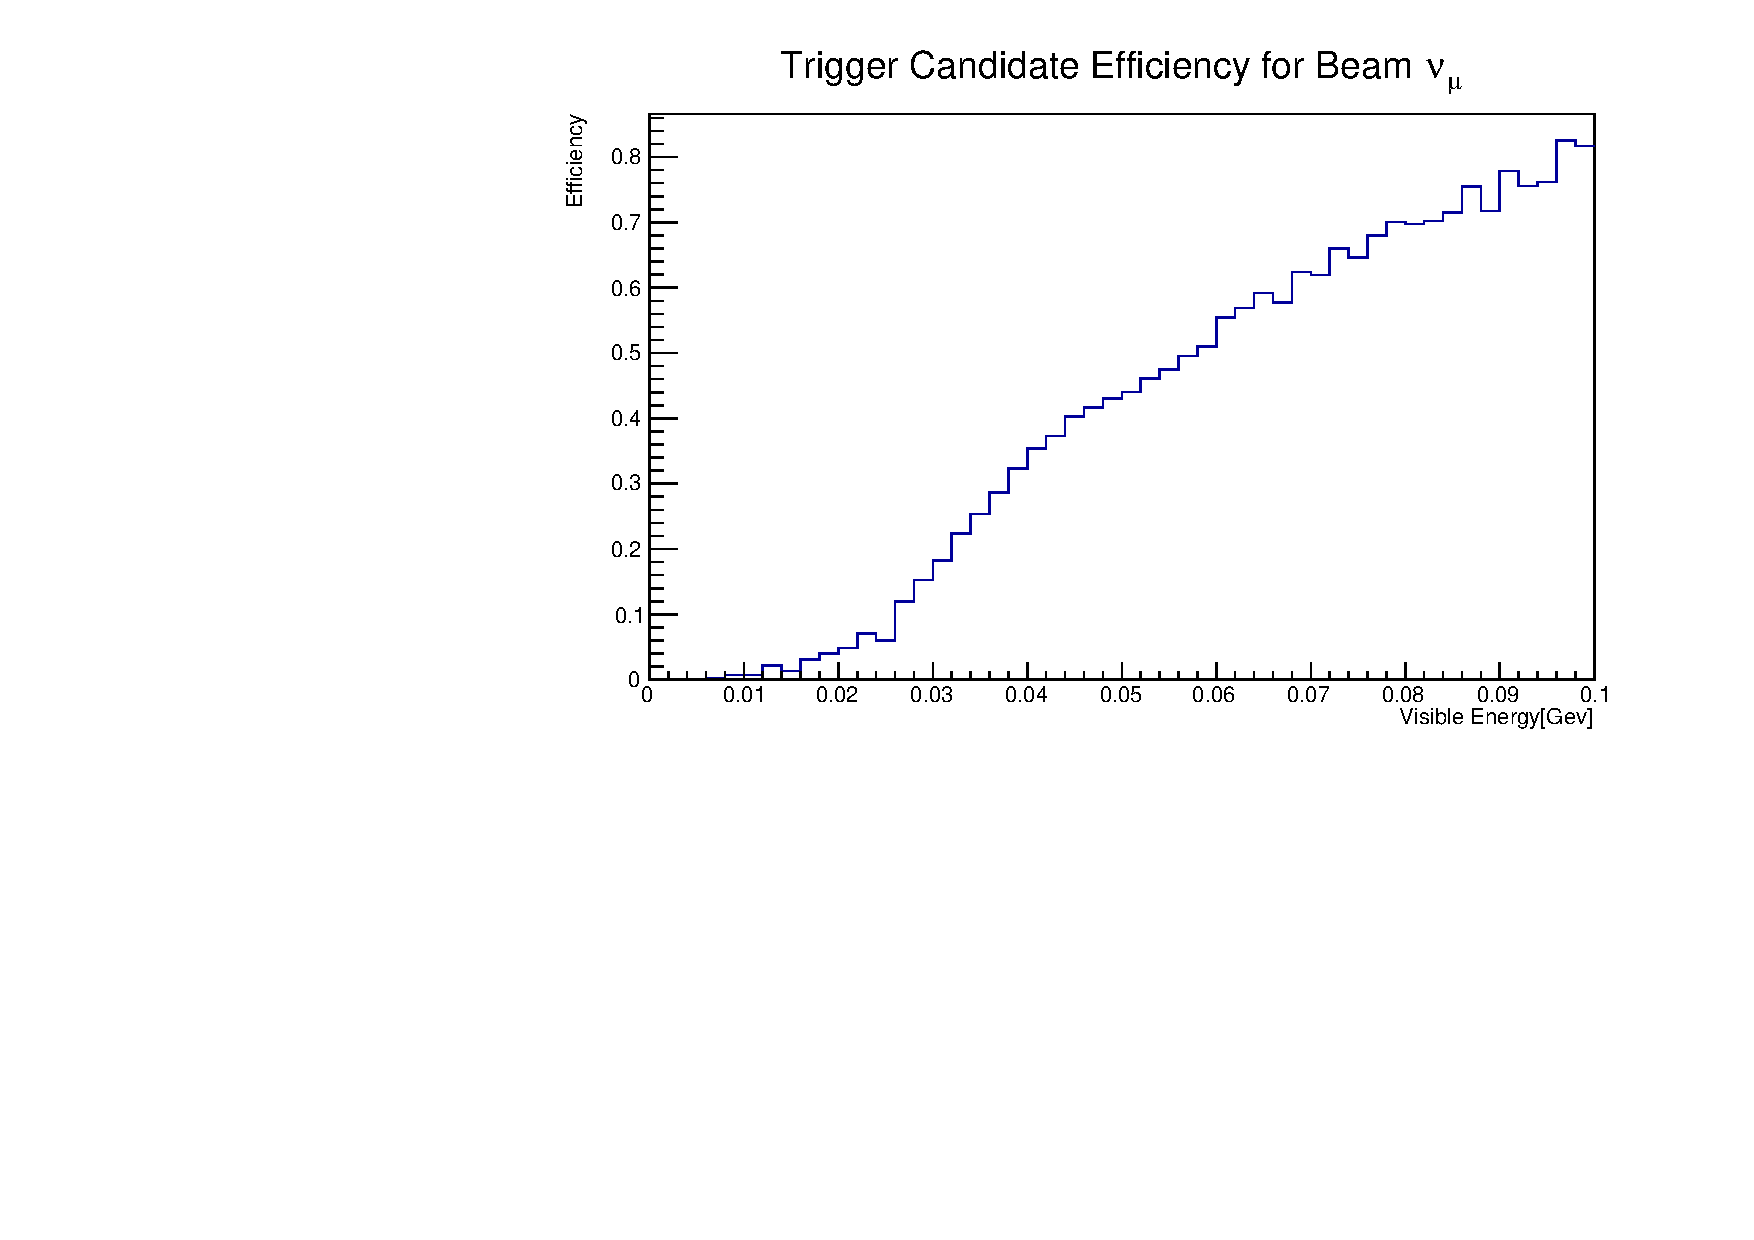
\includegraphics[angle=270,width=0.45\textwidth]{UpdatedEff/Differential_Nu_mu_Efficiency_MCC10.pdf}
    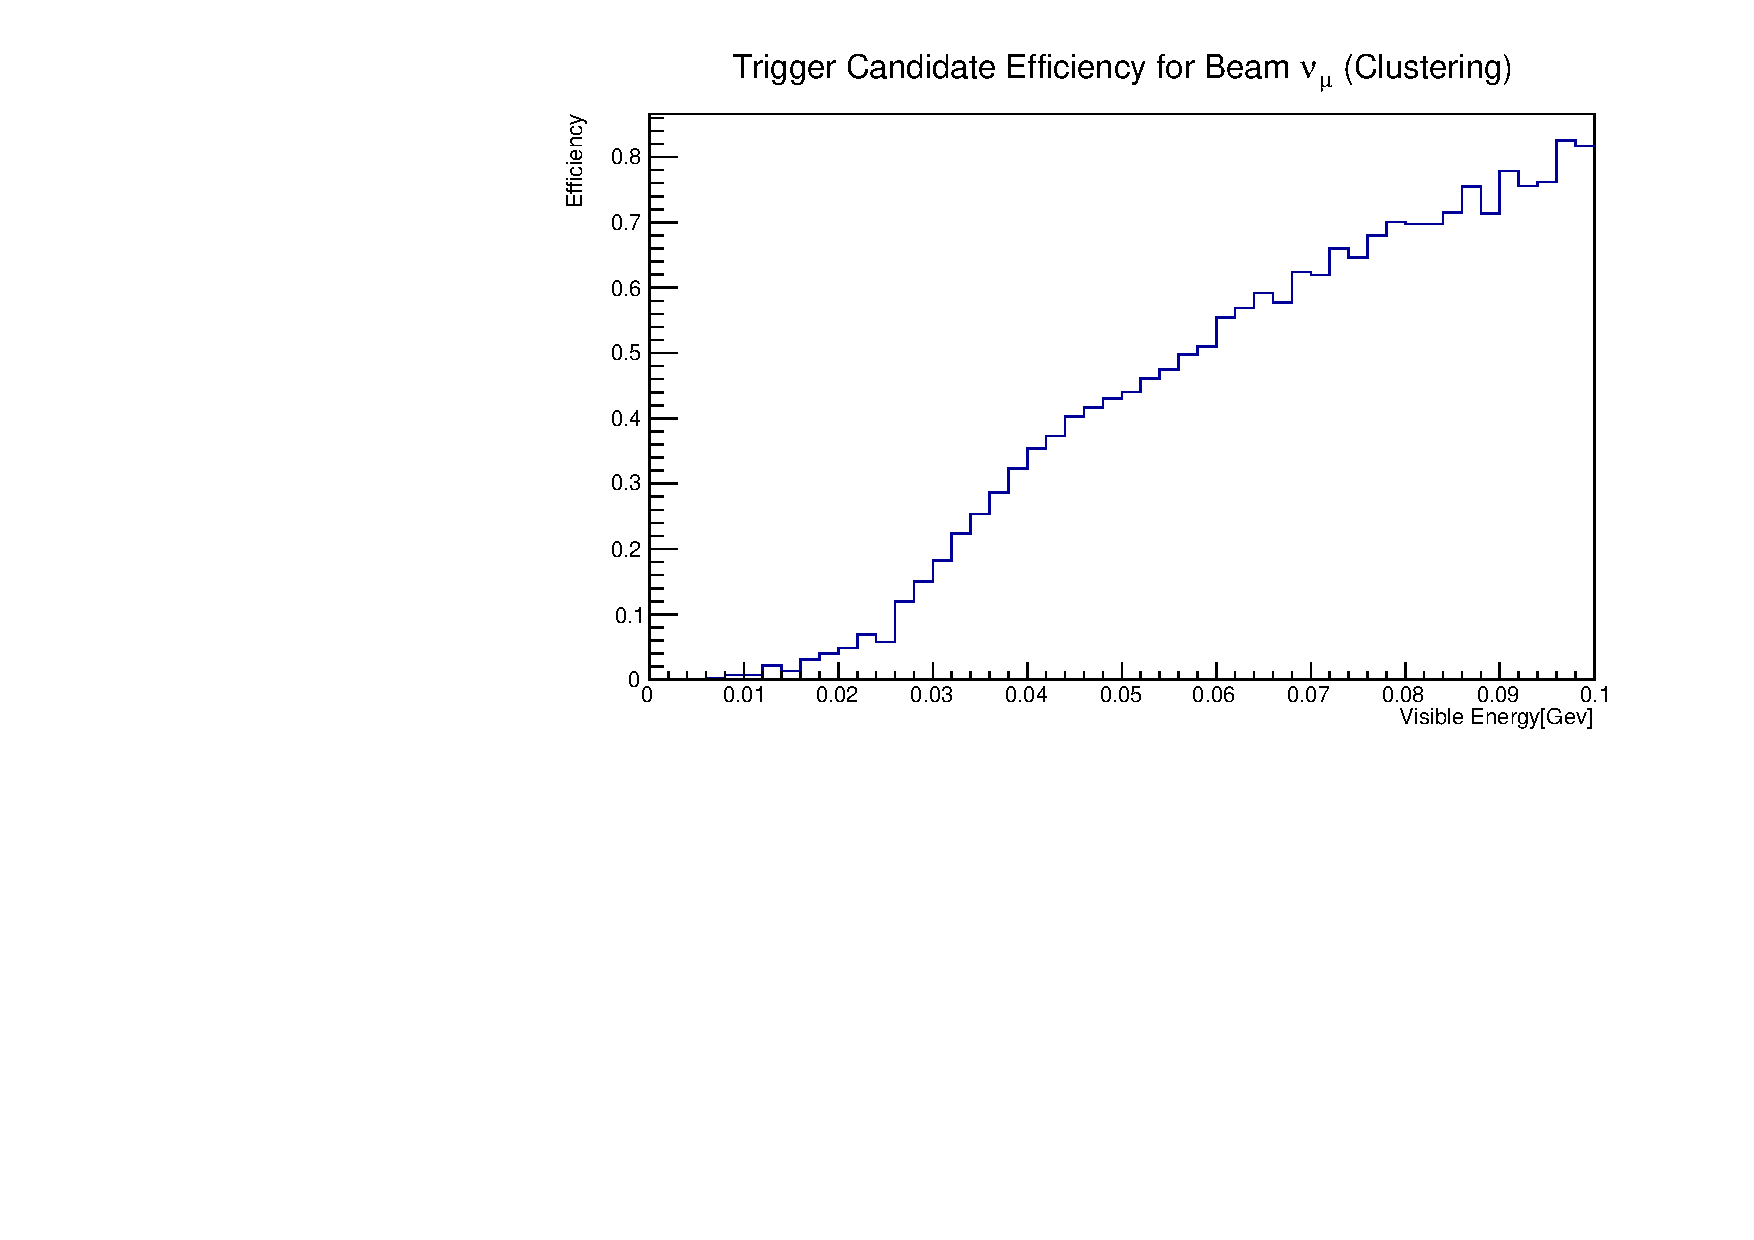
\includegraphics[angle=270,width=0.45\textwidth]{UpdatedEff/Differential_Nu_mu_Efficiency_MCC10_CLUS.pdf}
    \caption{Efficiency as a function of visible energy for un-oscillated Beam events from MCC10. Therefore, this sample is primarily $\nu_{\mu}$.}
    \label{fig:eff_beam_numu}
\end{figure}

\begin{figure}[H]
    \centering
    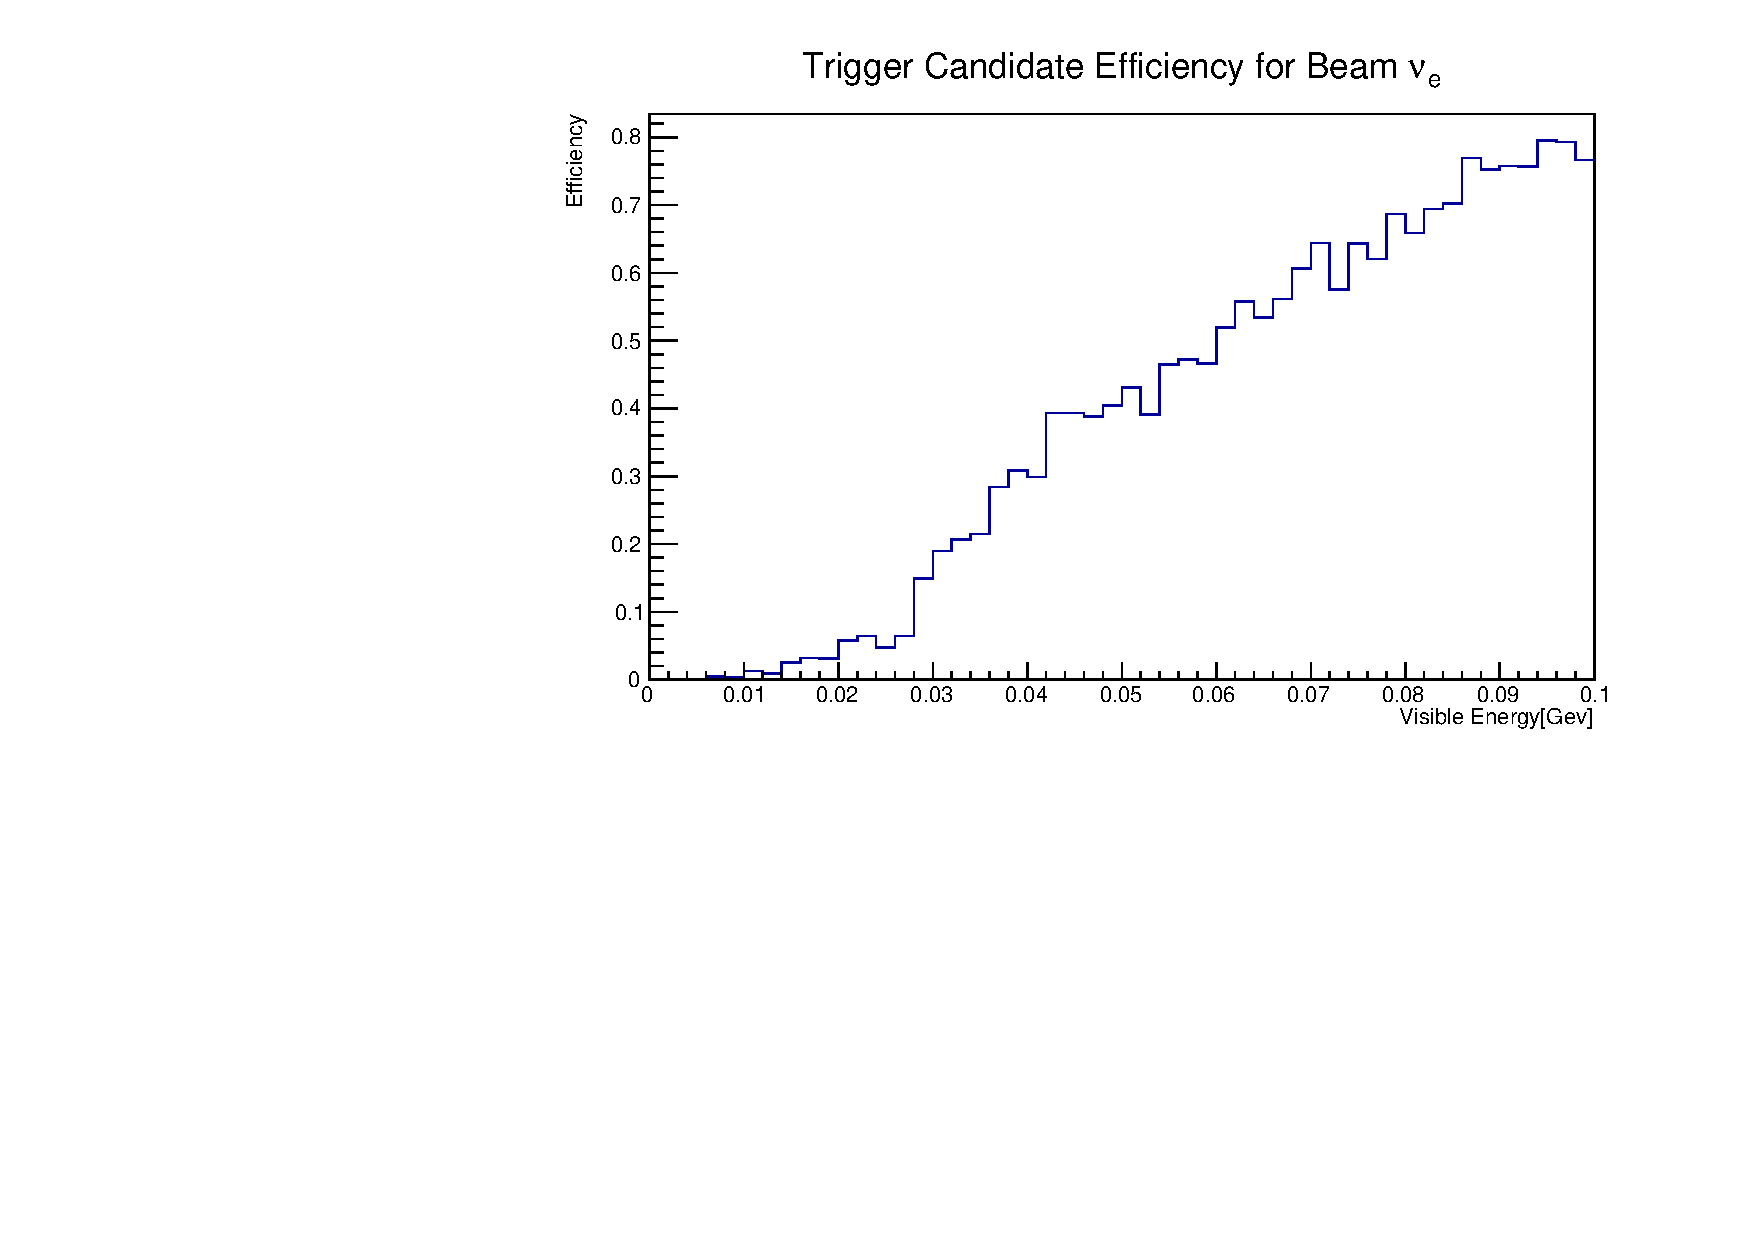
\includegraphics[angle=270,width=0.45\textwidth]{UpdatedEff/Differential_Nu_e_Efficiency_MCC10.pdf}
    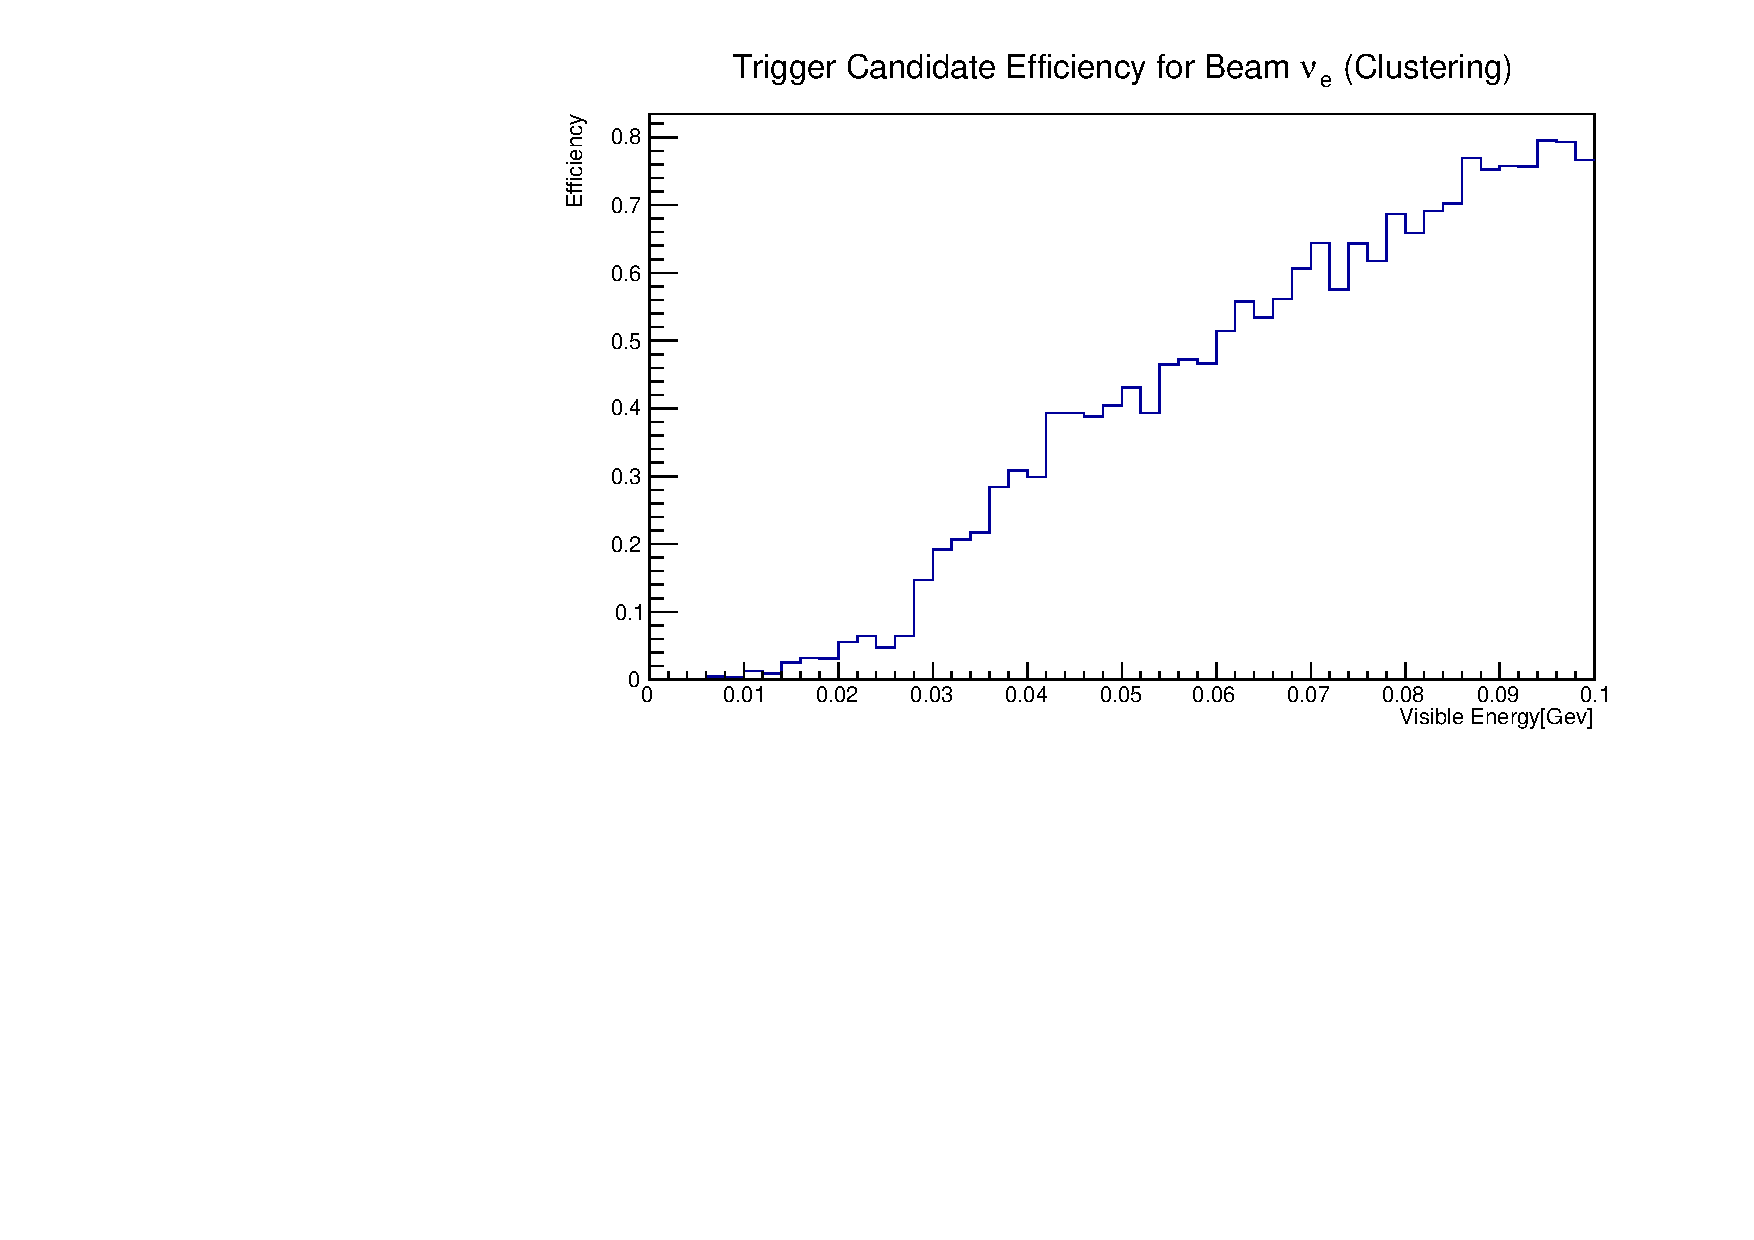
\includegraphics[angle=270,width=0.45\textwidth]{UpdatedEff/Differential_Nu_e_Efficiency_MCC10_CLUS.pdf}
    \caption{Efficiency as a function of visible energy for Beam events oscillated to $\nu_{e}$ from MCC10.}
    \label{fig:eff_beam_nue}
\end{figure}

As can be seen from the above, the differential efficiency is quite low due to the measured visible energy not necessarily being compact in the detector. The below show a better mark for the overall ability of the algorithm to trigger on any beam event.

\begin{figure}[H]
    \centering
    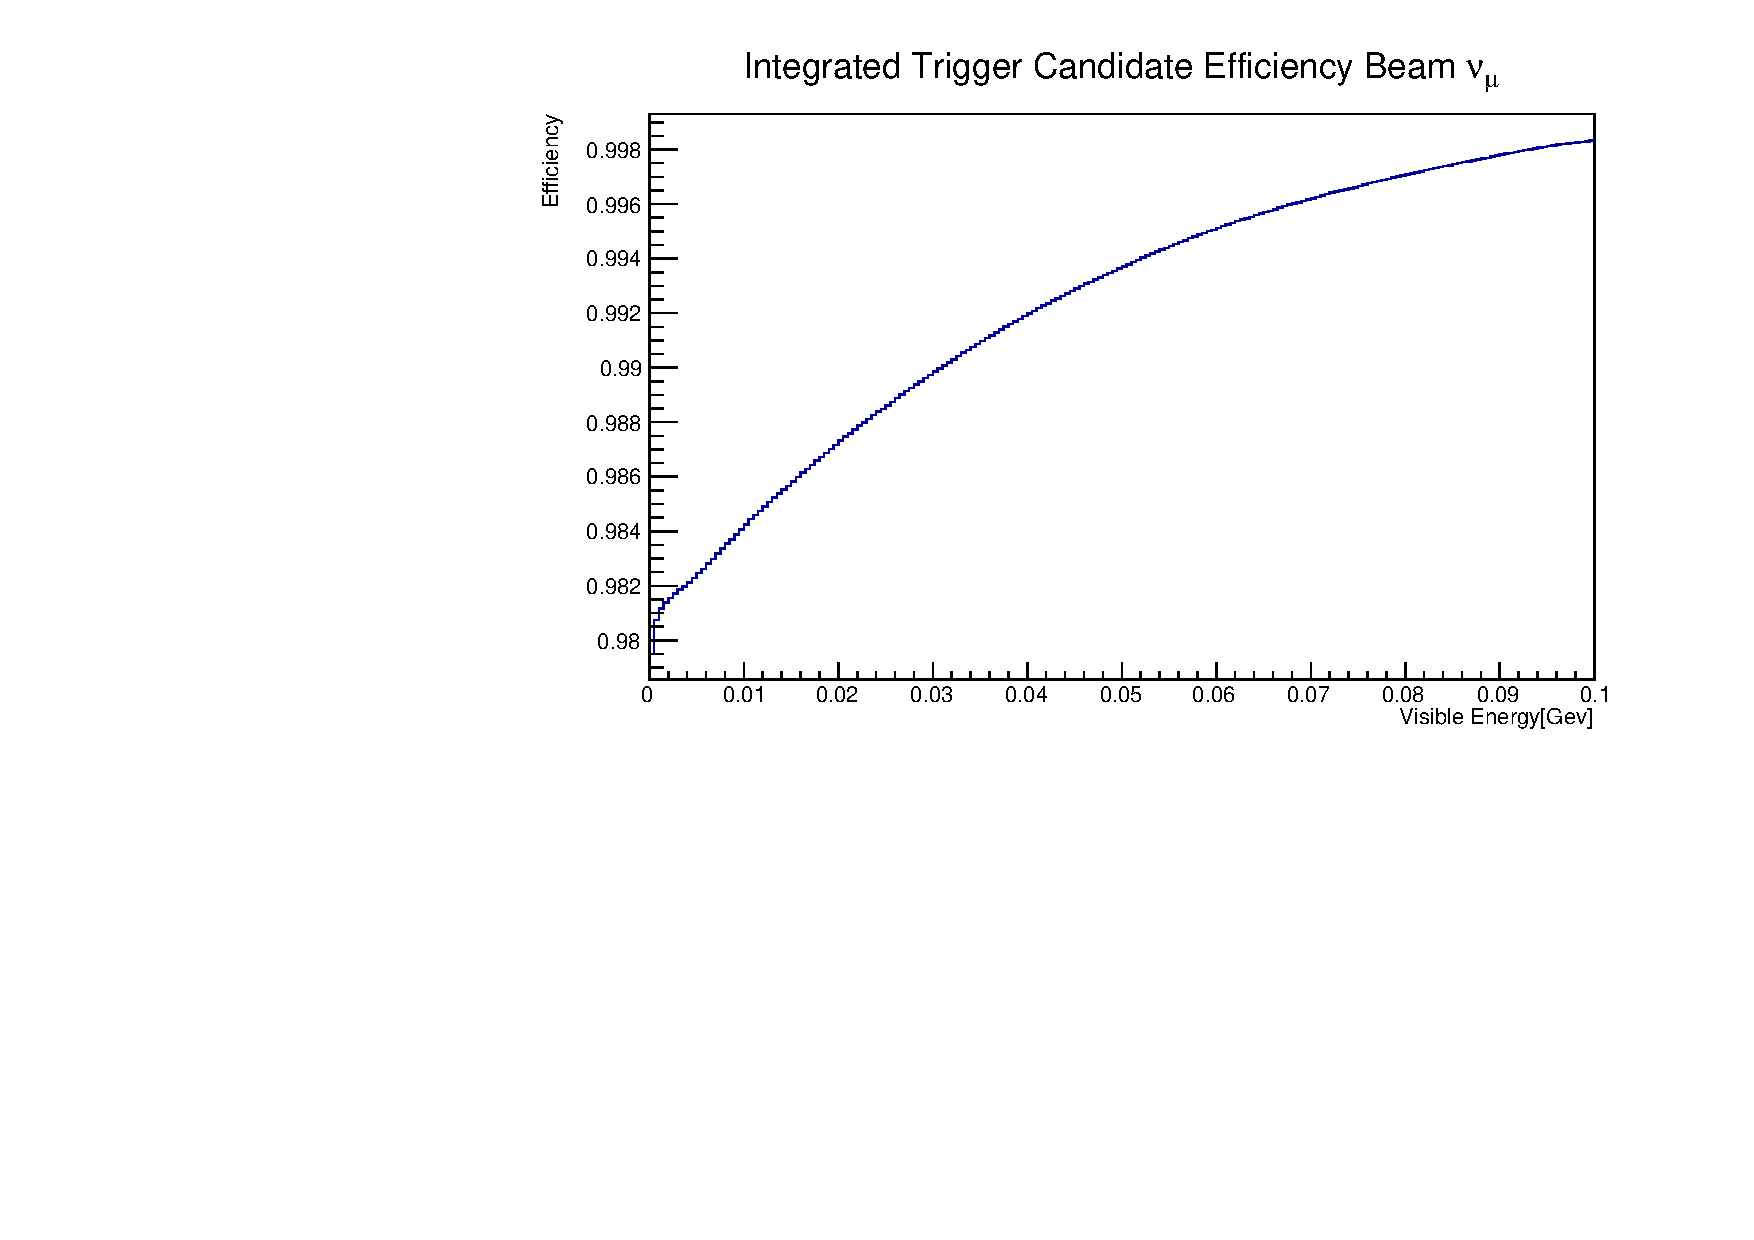
\includegraphics[angle=270,width=0.45\textwidth]{UpdatedEff/Integrated_Nu_mu_Efficiency_MCC10.pdf}
    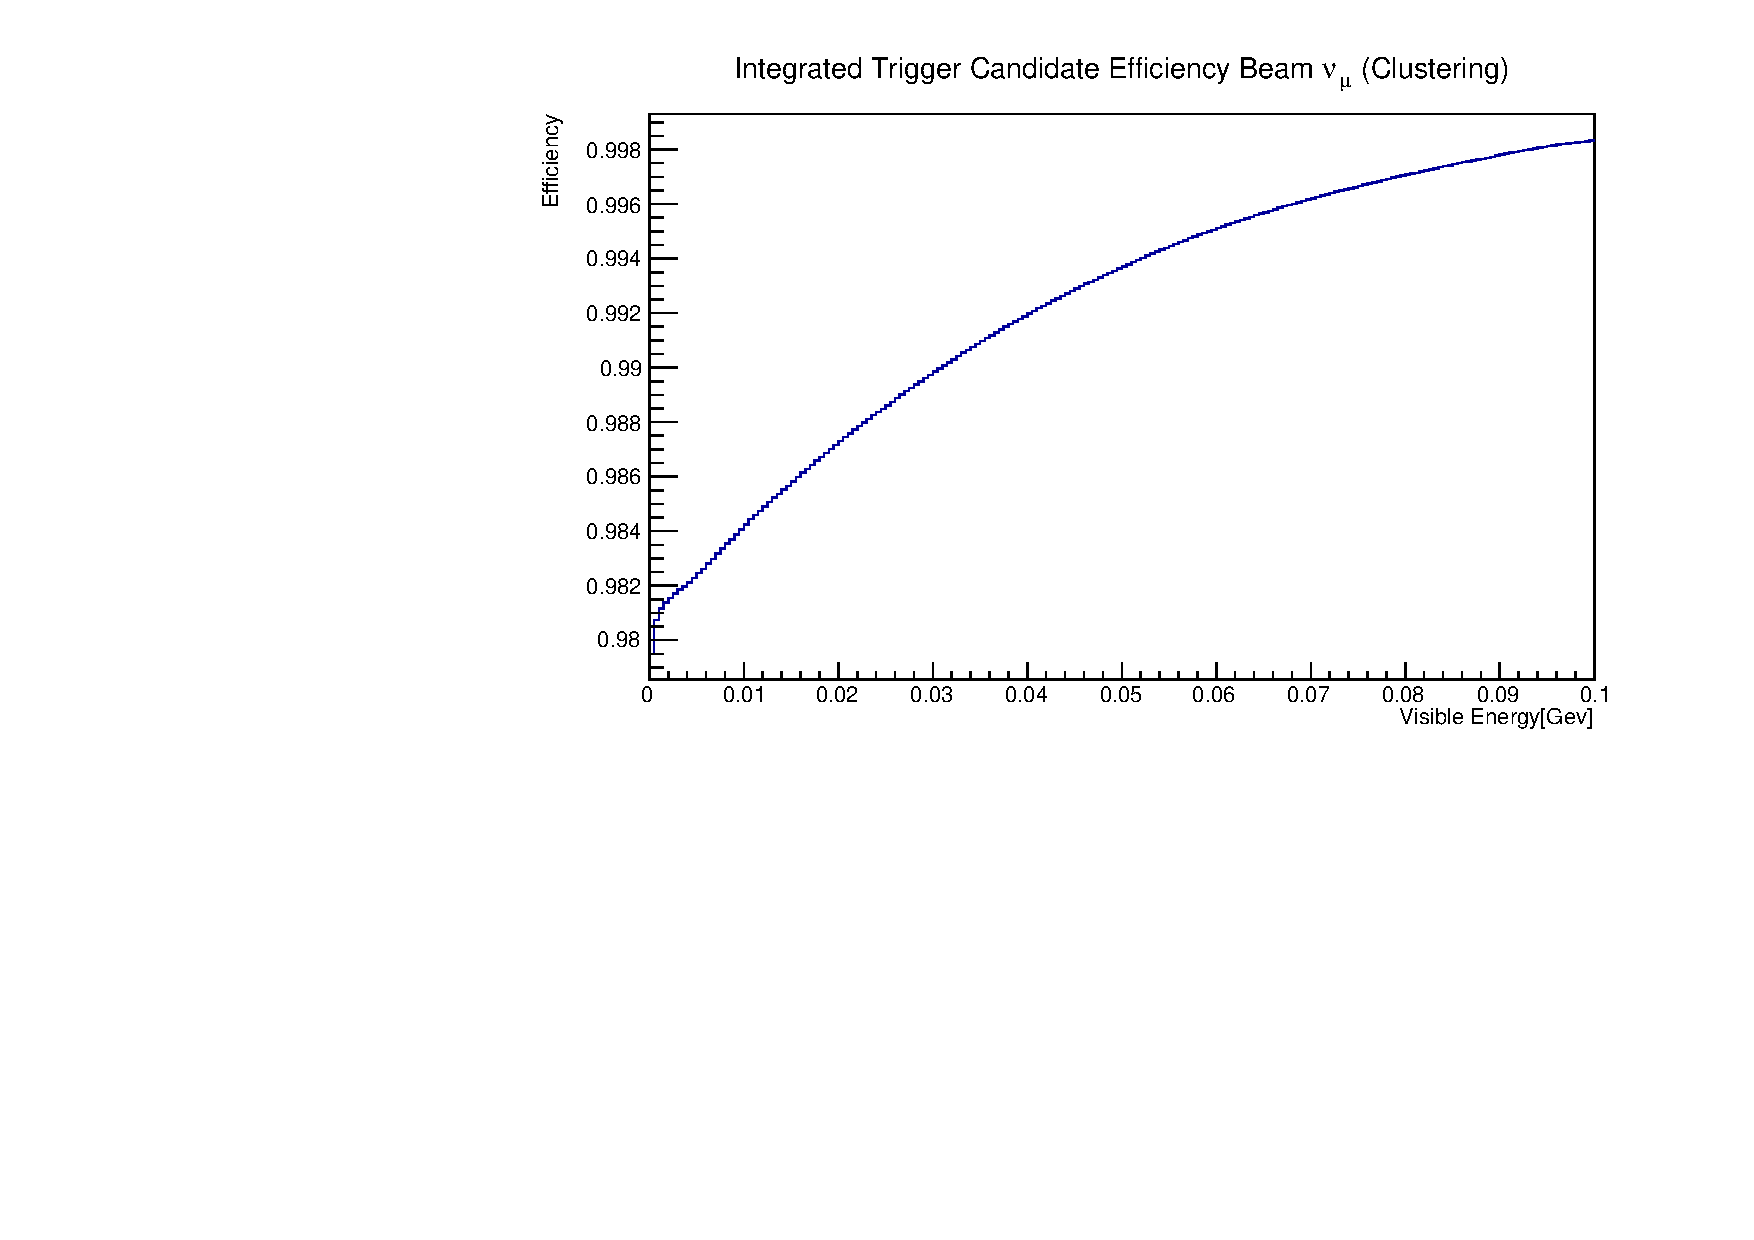
\includegraphics[angle=270,width=0.45\textwidth]{UpdatedEff/Integrated_Nu_mu_Efficiency_MCC10_CLUS.pdf}
    \caption{Efficiency to issue a candidate at or above the given visible energy for un-oscillated Beam events from MCC10. Therefore, this sample is primarily $\nu_{\mu}$.}
    \label{fig:eff_beam_numu_int}
\end{figure}

\begin{figure}[H]
    \centering
    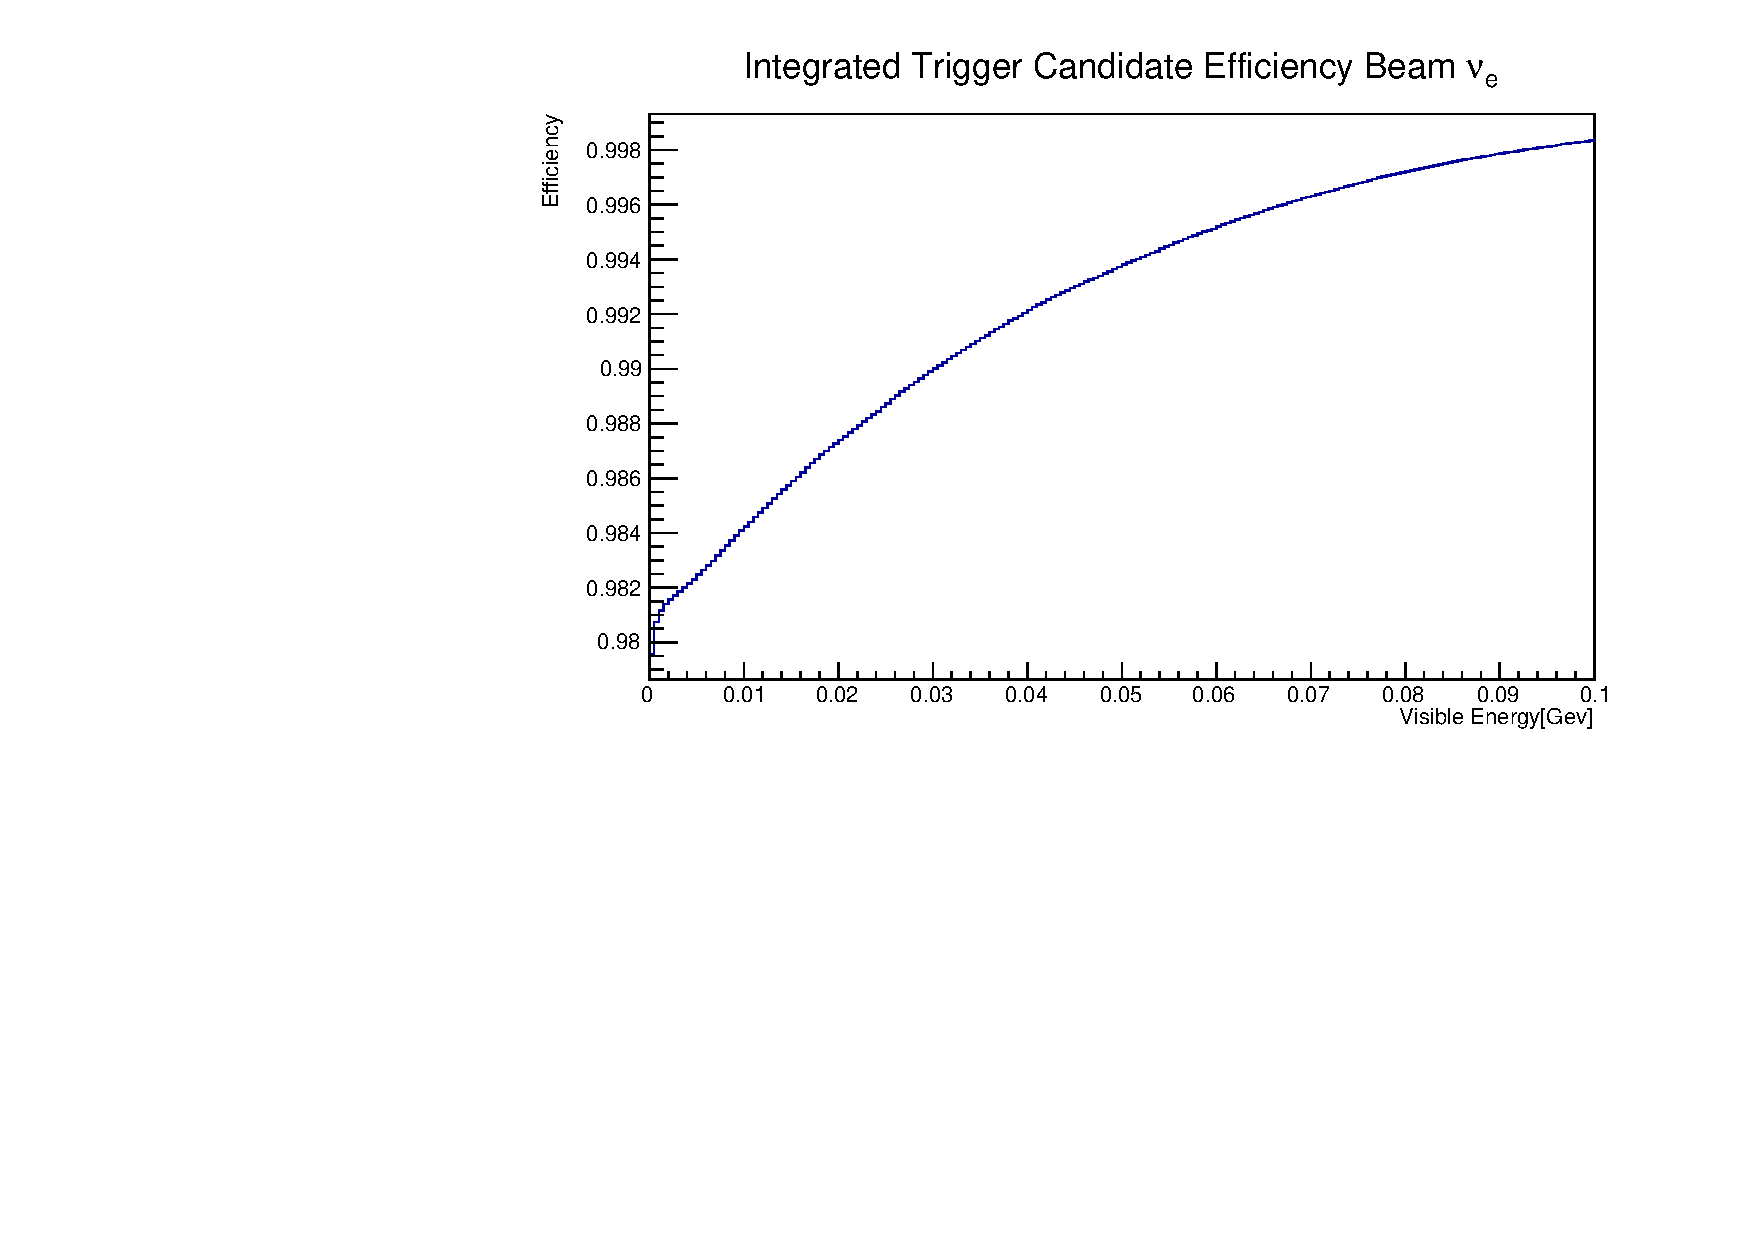
\includegraphics[angle=270,width=0.45\textwidth]{UpdatedEff/Integrated_Nu_e_Efficiency_MCC10.pdf}
    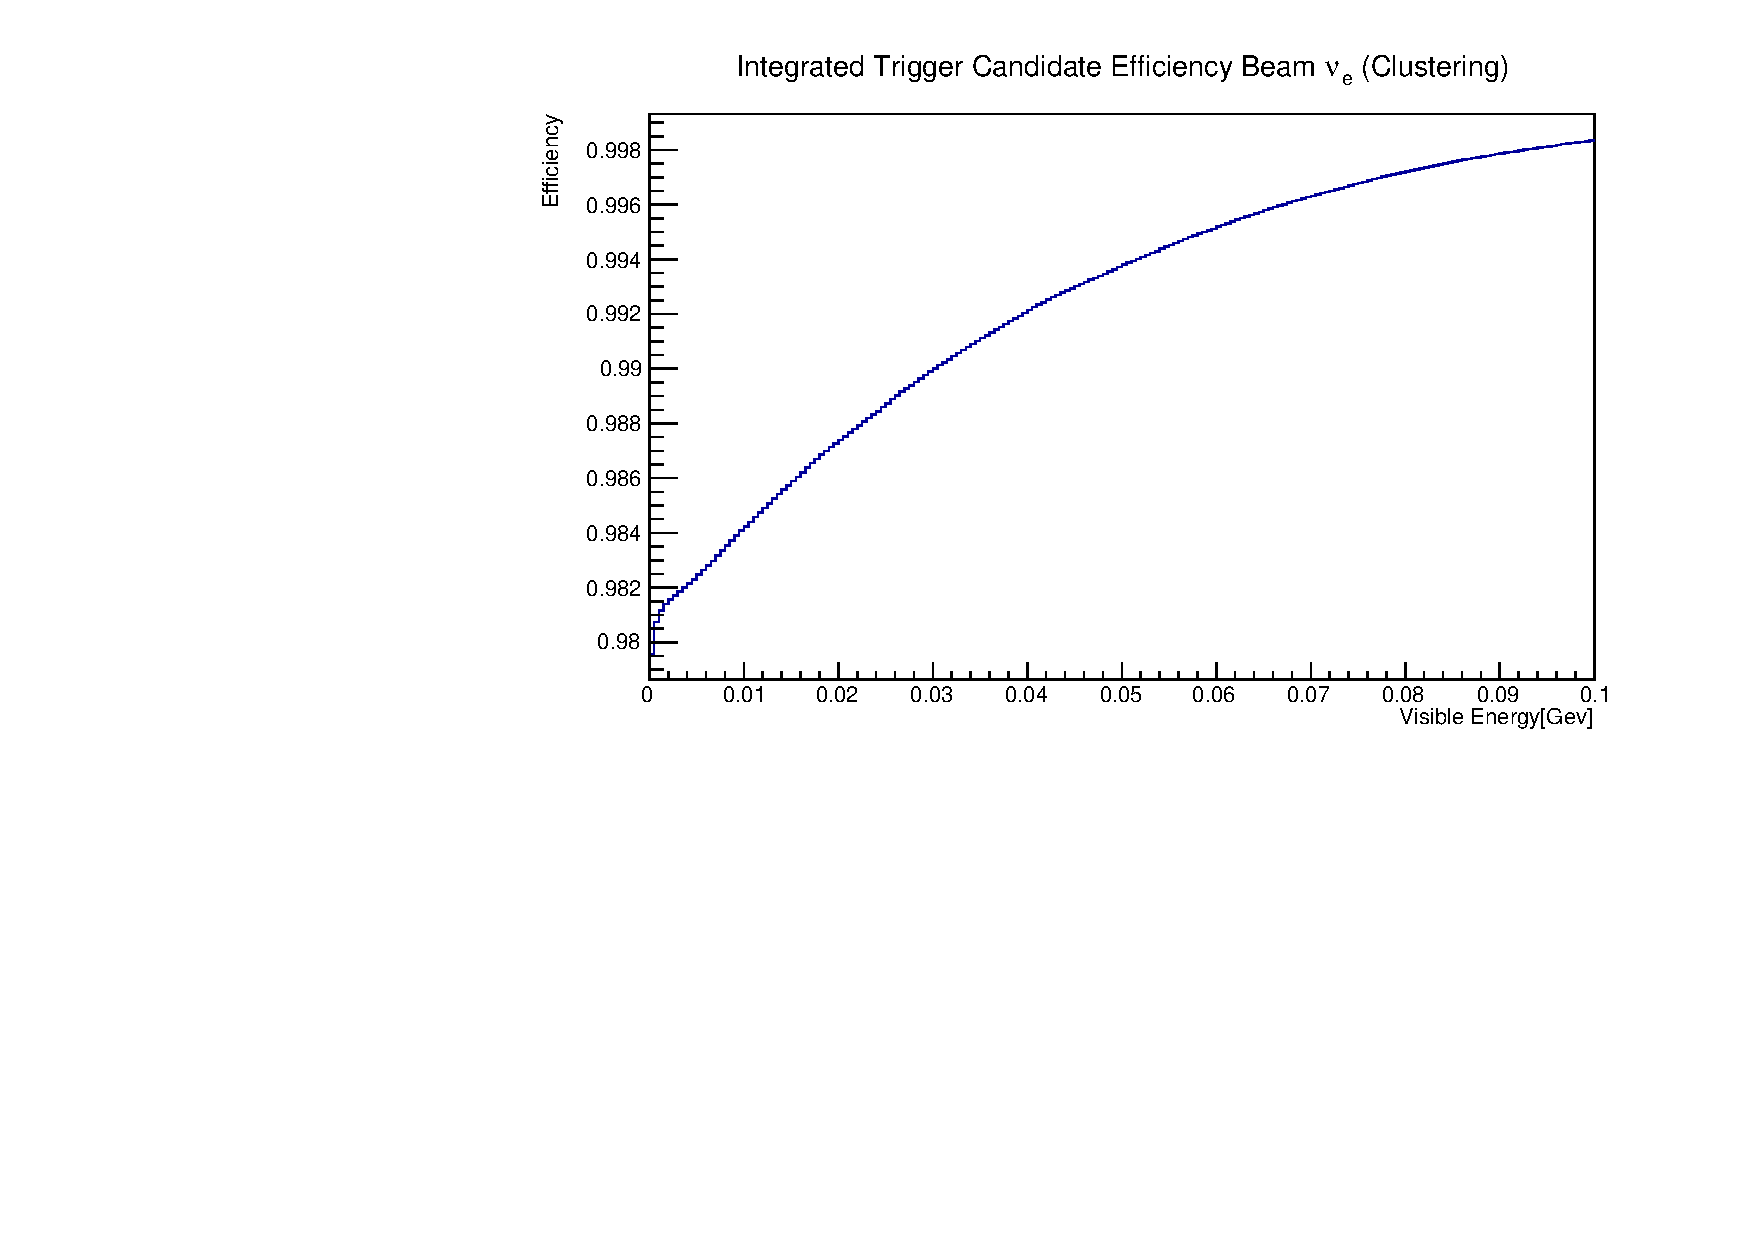
\includegraphics[angle=270,width=0.45\textwidth]{UpdatedEff/Integrated_Nu_e_Efficiency_MCC10_CLUS.pdf}
    \caption{Efficiency to issue a candidate at or above the given visible energy for Beam events oscillated to $\nu_{e}$.}
    \label{fig:eff_beam_nue_int}
\end{figure}

\subsubsection{Atmospherics MCC}

The following shows the trigger efficiency as a function of visible energy for the MCC9 sample of atmospheric events. The integrated efficiency is included for the same reason as above.


\begin{figure}[H]
    \centering
    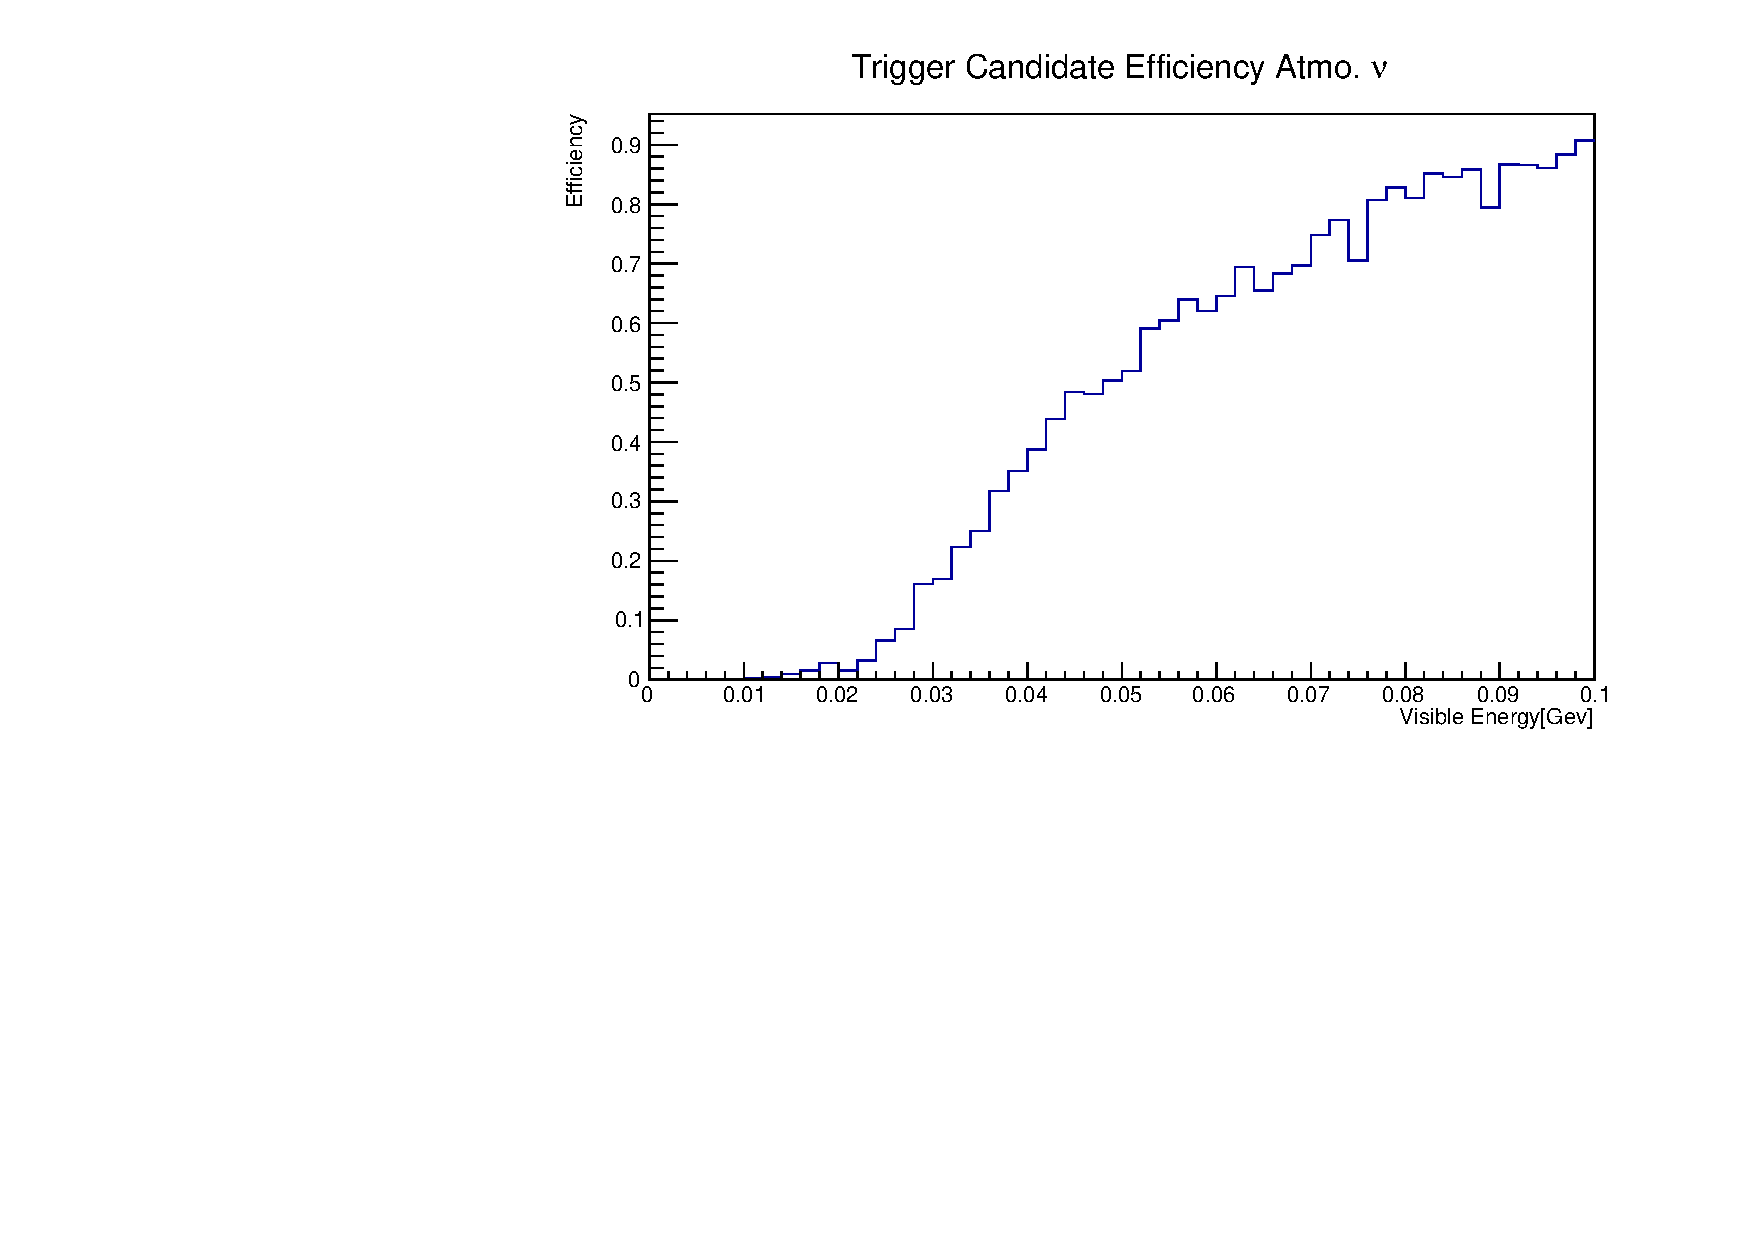
\includegraphics[angle=270,width=0.45\textwidth]{UpdatedEff/Differential_Atmnu_Max_Efficiency_MCC9.pdf}
    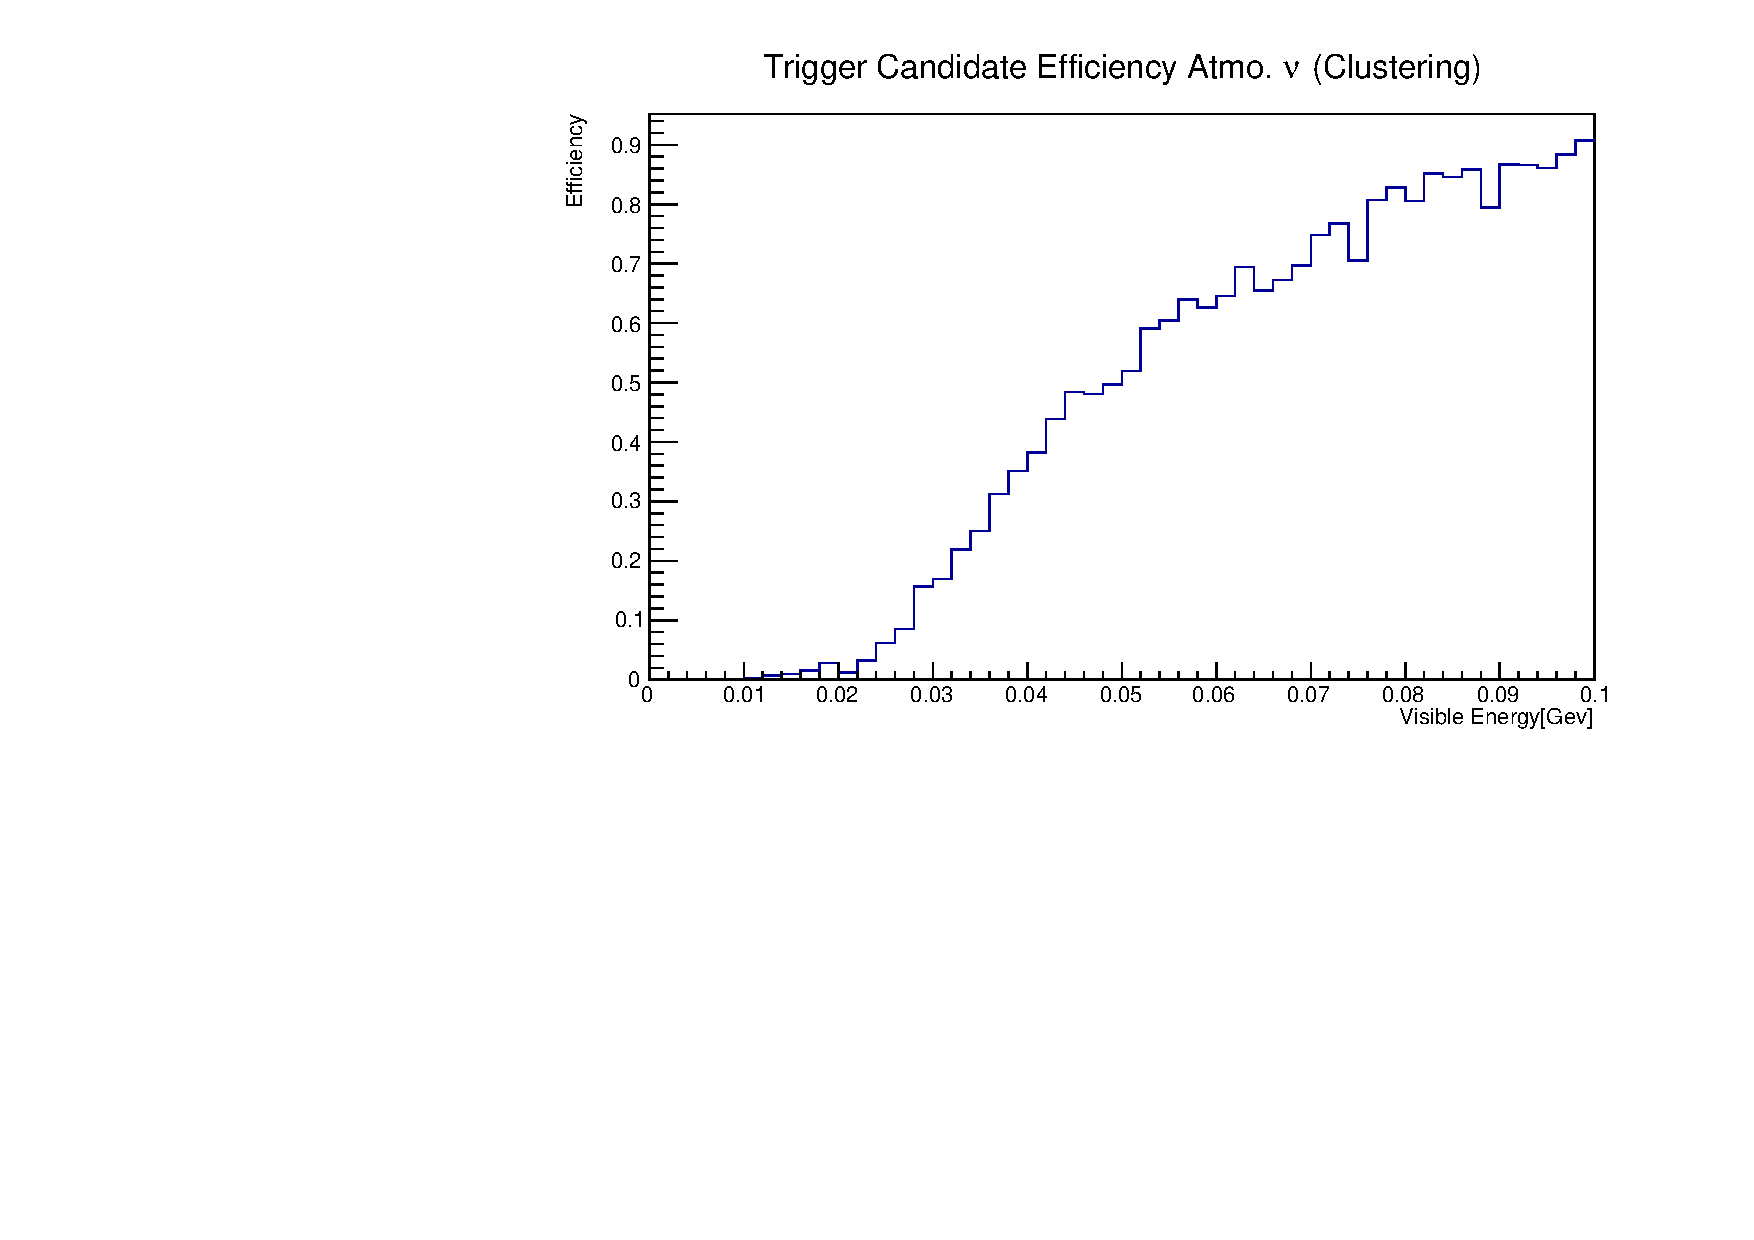
\includegraphics[angle=270,width=0.45\textwidth]{UpdatedEff/Differential_Atmnu_Max_Efficiency_MCC9_CLUS.pdf}
    \caption{Efficiency as a function of visible energy for simulated Atmoshperic Events with Maximum Bartol Flux from MCC9}
    \label{fig:eff_atm}
\end{figure}

\begin{figure}[H]
    \centering
    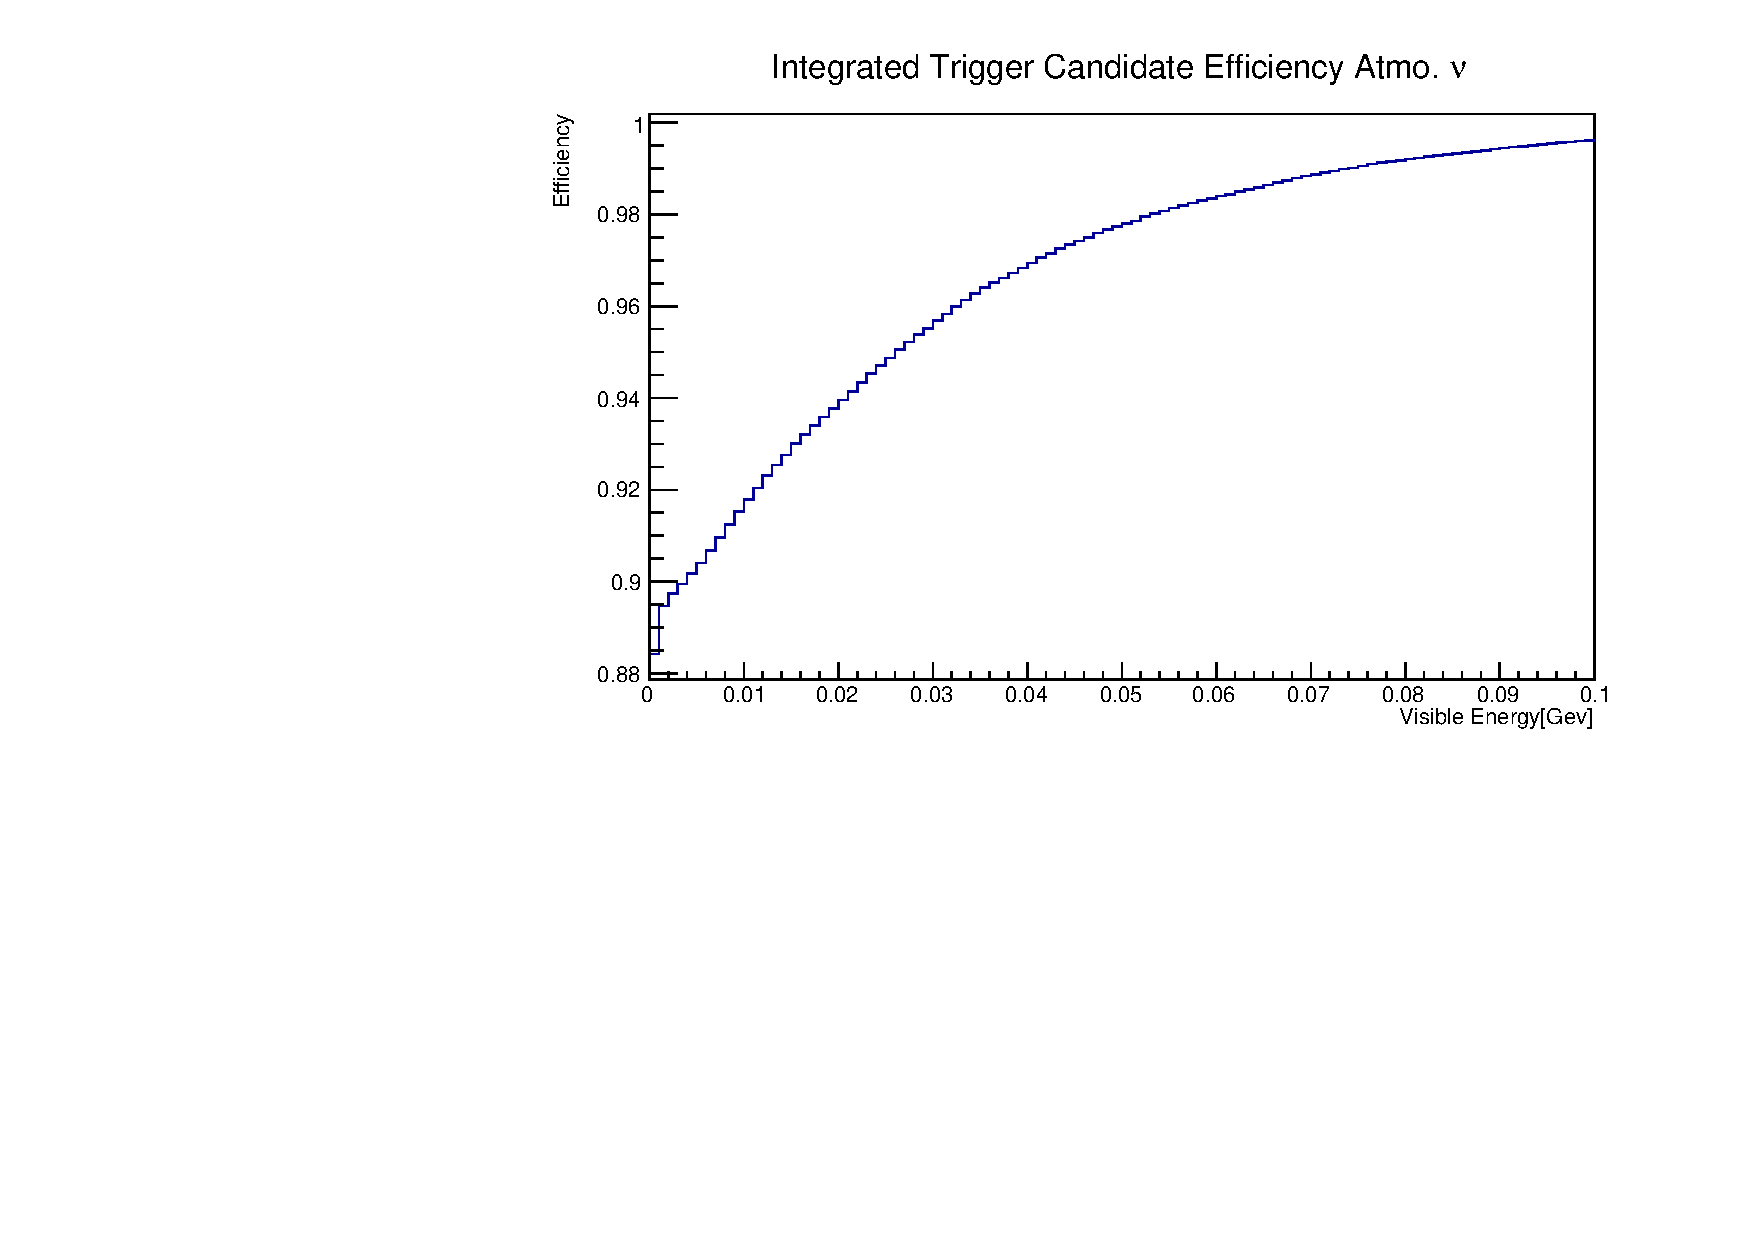
\includegraphics[angle=270,width=0.45\textwidth]{UpdatedEff/Integrated_Atmnu_Max_Efficiency_MCC9.pdf}
    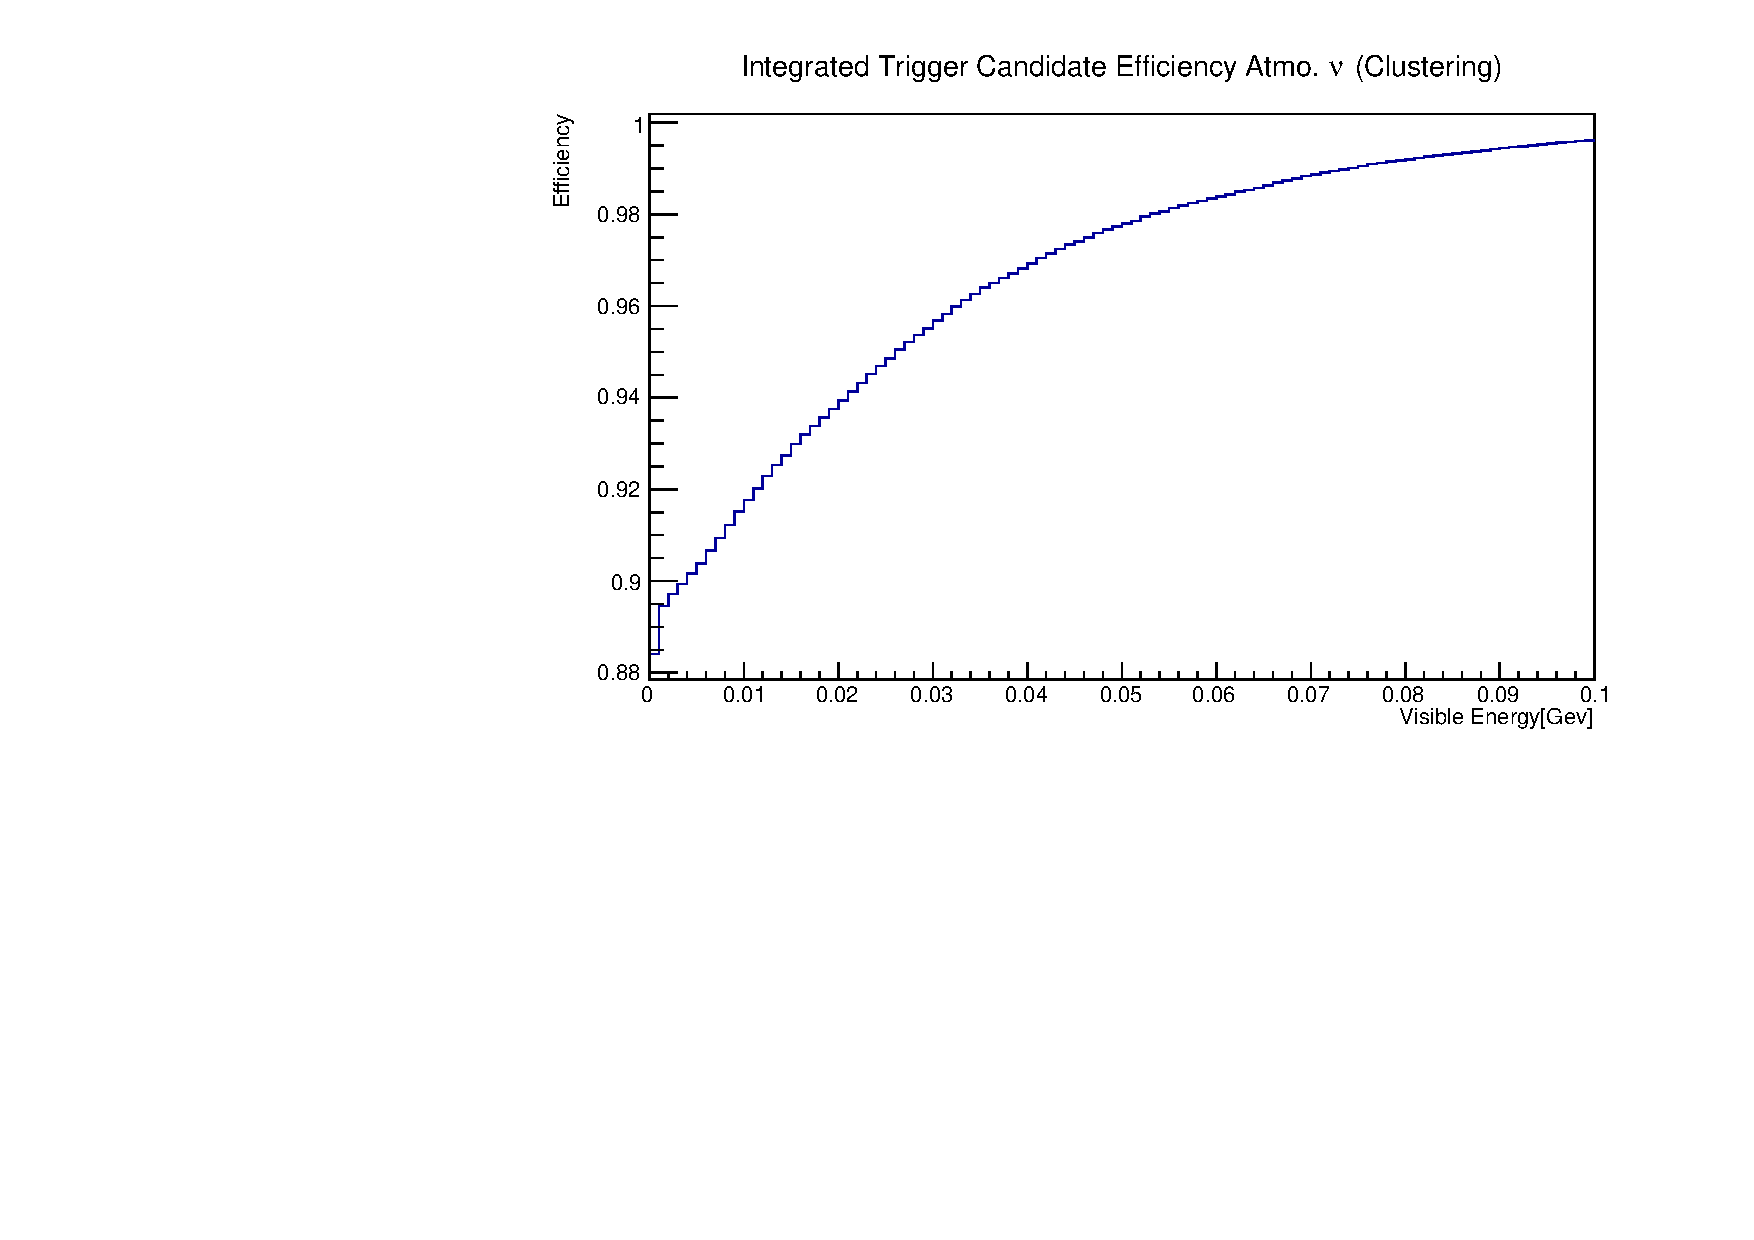
\includegraphics[angle=270,width=0.45\textwidth]{UpdatedEff/Integrated_Atmnu_Max_Efficiency_MCC9_CLUS.pdf}
    \caption{Efficiency to issue a candidate at or above a given visible energy for simulated Atmoshperic Events with Maximum Bartol Flux from MCC9}
    \label{fig:eff_atm_int}
\end{figure}

\subsubsection{Single Electron Trigger Efficiency}
A 1-100 MeV, isotropic, electron sample without radiological backgrounds was generated to demonstrate the trigger efficiency for events resulting in daughter electrons of this energy range. The following results stand as a measure of the algorithms' handling of energy deposits from electrons, which inherently makes them a measure of the algorithms' handling of compact energy deposits.

\begin{figure}[H]
    \centering
    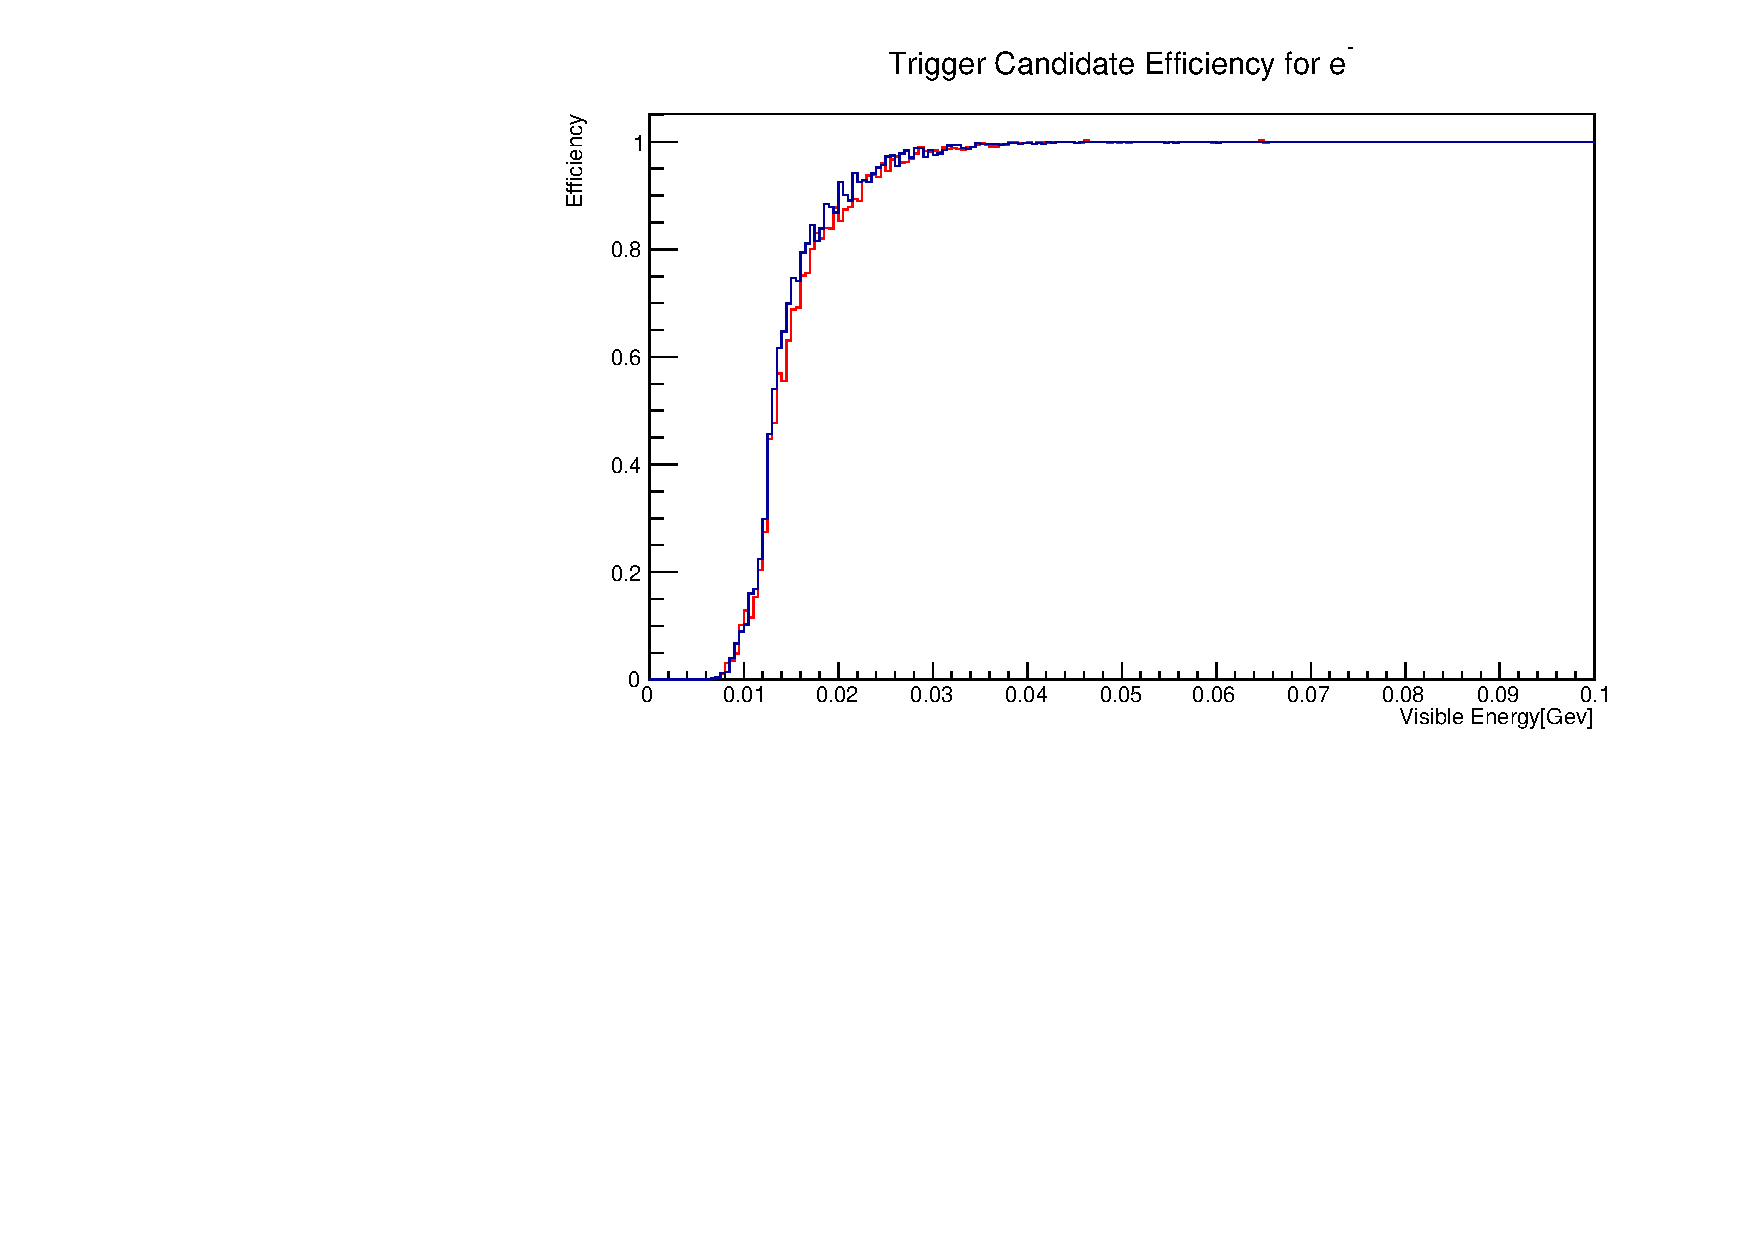
\includegraphics[angle=270,width=0.65\textwidth]{UpdatedEff/Electron_Efficiency_Comparison.pdf}
    \caption{Efficiency to issue a candidate as a function of visible energy for simulated electrons without backgrounds for two methods of primitive generation, offline (red) and online (blue).}
    \label{fig:eff_electron}
\end{figure}

\subsection{Algorithm Benchmarks}

To ensure that the algorithms meet the timing constraints imposed by the limited buffer capabilities under normal streaming conditions for TPC data, the process for generating the trigger candidates, after being passed hit objects from an event, was timed. Tables~\ref{tab:bench_adj} and \ref{tab:bench_clustering} below are a summary of the average processing time for the various samples when executed on a single core process. 

%TODO:mention that this is for single threshold of 15 ADC

\begin{table}[H]
\begin{center}
\caption{Adjacency Algorithm}
%\begin{tabular}{ |l|l|l|l|l|l| }
\begin{tabulary}{\textwidth}{ |l|l|l|l|l|l| }
  \toprule
  \rowtitlestyle Sample & \textnumero\;of Evt. & \textnumero\;of APA & \textnumero\;of APA Windows & APA Data Time & Processing Time \\ 
  \toprowrule 
  Beam          & 945,500 & 12 & 11,346,000 & 424.72m & 592.97s   \\ \colhline %reduction:42.98
  Atmospherics  & 99,800  & 12 & 1,197,000  & 44.83m  & 16.26s    \\ \colhline %reduction:165.43
  Radiologicals & 103,000 & 1  & 103,000    & 3.85m   & 15.35s    \\ \colhline %reduction:15.03
\end{tabulary}
%\caption{Adjacency Algorithm}
\label{tab:bench_adj}
\end{center}
\end{table}

\begin{table}[H]
\begin{center}
\caption{Clustering Algorithm}
\begin{tabulary}{\linewidth}{ |l|l|l|l|l|l| }
  \toprule
  \rowtitlestyle Sample & \textnumero\;of Evt. & \textnumero\;of APA & \textnumero\;of APA Windows & APA Data Time & Processing Time \\ 
  \toprowrule 
  Beam          & 945,500 & 12 & 11,346,000 & 424.72m  & 1367.73s  \\ \colhline %reduction:18.63
  Atmospherics  & 99,800  & 12 & 1,197,600  & 44.83m   & 40.31s    \\ \colhline %reduction:66.55
  Radiologicals & 103,000 & 1  & 103,000    & 3.85m    & 51.26s    \\ \colhline %reduction:4.51
  %\bottomrule
\end{tabulary}
%\caption{Clustering Algorithm}
\label{tab:bench_clustering}
\end{center}
\end{table}



%%%% FIXME: This is the paragraph that felt outdated... changing this I think will be all that's necessary in this section...
Cutting solely on the ``keep-all" thresholds, the efficiency curves do not meet the necessary requirements. An improvement is expected from the implementation of multi-dimensional selection.

Closer inspection of the events that led to efficiency loss suggest that these are primarily neutral-current quasi-elastic interactions. Work is in progress to understand how to better trigger on these events, the primary issue being difficulty of triggering on neutron-laden final states. It should be noted that neutron interactions in Argon are still an open area of study and future results in this area will improve the ability to understand how to trigger on them.

Given that the radiological activity will be a constant sink of the allotted processing time, we can take the reduction factor for the candidate-production algorithms in the radiological sample as a baseline. This reduction factor is the ratio of APA Data Time to Processing Time i.e. 15.03 for the Adjacency-based algorithm vs. 4.51 for the clustering algorithm.  

Comparison of the two different hit-grouping methods points towards Adjacency being the optimal option, due to its faster processing time, and no noticeable differences between the distributions for radiologicals. It is possible that Clustering may be more robust against pile-up and therefore necessary in the presence of increased radiological rates. 

\end{document}
